\documentclass[preprint,12pt]{elsarticle}

\usepackage{amsmath}
\usepackage{amsfonts}
\usepackage{amssymb}
\usepackage{draftwatermark}
\usepackage{tabularx} % Required for tables that stretch to text width
\usepackage{booktabs} % For prettier tables
\usepackage{ltablex}
\usepackage{xcolor,cancel,bm,tikz}
\usepackage{hyperref}
\usepackage{mathtools}
\usepackage{amsmath,amssymb,amsthm,amsfonts}
\usepackage{enumitem}
\usepackage{kantlipsum,graphicx}
\usepackage{multicol,colortbl,multirow}
\usepackage{pgfplots,booktabs,xfrac,floatrow}
\usepackage{color}
\usepackage{titlesec}
\usepackage{natbib}


\titleformat*{\section}{\Large\bfseries}
\titleformat*{\subsection}{\normalsize\bfseries}
\titleformat*{\subsubsection}{\normalsize\bfseries}
\numberwithin{equation}{section}

\usepackage{setspace}
\setstretch{0.7} % Adjust this value as needed

\setlength{\parindent}{0pt}

\usepackage{geometry}
\geometry{
  left=1in,
  right=1in,
  top=1in,
  bottom=1in,
}

\SetWatermarkText{DRAFT}
\SetWatermarkScale{1}


\journal{Mathematical and Computer Modelling}


\begin{document}

\begin{frontmatter}

\title{Validity of a model for a cantilever two-dimensional beam}

\author{Rudi du Toit}
\address{University of Pretoria, Pretoria, South Africa}

\begin{abstract}
Your abstract here.
\end{abstract}

\begin{keyword}
Vibration \sep Cantilever \sep Beam \sep Three-Dimensional \sep Two-Dimensional
\end{keyword}

\end{frontmatter}

\section{Introduction}
Your introduction here.

\section{Models}

\subsection{Three-dimensional model}
Consider a vector valued displacement function $u \in \Omega \subset R^3$.

\subsubsection*{Equation of motion}\label{ssec:3D_Model:EquationOfMotion}
\begin{eqnarray}
	\rho\partial_t^2 u & = & \textrm{div}T + Q. \label{eq:3D_Model:EM}
\end{eqnarray} \label{sym:rho} \label{sym:partial_diff} \label{sym:T} \label{sym:Q}

Here $\rho$ is the density, $T$ is the stress tensor, and $Q$ is the external 
force per unit volume and $\textrm{div}T$ is the divergence of the tensor $T$ and represented by
\begin{eqnarray}
	\textrm{div}  T & = &
	\begin{bmatrix}
		\partial_1 \sigma_{11} + \partial_2 \sigma_{12} + \partial_3 \sigma_{13} \\
		\partial_1 \sigma_{21} + \partial_2 \sigma_{22} + \partial_3 \sigma_{23} \\
		\partial_1 \sigma_{31} + \partial_2 \sigma_{32} + \partial_3 \sigma_{33}
	\end{bmatrix}. \label{eq:3D_Model:divT}
\end{eqnarray}

Assuming only small vibrations, the stress tensor $T$ is symmetric due to small
local displacements and rotations. The trace of the stress tensor $T$ is denoted
\begin{eqnarray}
	\textrm{Tr}(T) & = & \sigma_{11} + \sigma_{22} + \sigma_{23}. \label{eq:stress_tensor_t}
\end{eqnarray}

\subsubsection*{Constitutive Equation}
For an isotropic material, Hooke's law can be written in terms of Young's modulus $E$ and Poisson's ratio $\nu$ as follows.\\

\textit{Hooke's law}
\begin{eqnarray}
	\mathcal{E} = \left( \frac{1+\nu}{E} \right)T - \frac{\nu}{E}\textrm{Tr}(T)I,  \label{eq:3D_Model:HL}
\end{eqnarray} The components of the strain tensor $\mathcal{E}$ are defined as
\begin{eqnarray}
	\varepsilon_{ij} = \frac{1}{2}\left( \frac{\partial u_i}{\partial x_j} + \frac{\partial u_j}{\partial x_i} \right). \label{eq:3D_Model:Strain}
\end{eqnarray}\label{sym:varepsilonij}

If the principal stresses $\sigma_i$ are all non-zero, then Hooke's law can be written in an alternative form.\\

\textit{Hooke's law in the alternative form}
\begin{eqnarray}
	T = \left( \frac{E}{1+\nu} \right)\mathcal{E} + \frac{\nu E}{(1+\nu)(1-2\nu)}\textrm{Tr}(\mathcal{E})I \label{eq:3D_Model:CE}.
\end{eqnarray}
With $\textrm{Tr}(\mathcal{E}) = \epsilon_{11} + \epsilon_{12} + \epsilon_{13}$ is the trace of the strain operator $\mathcal{E}$.\\

In this form, Hooke's law is the constitutive equation for the three-dimensional model.

\subsection{Dimensionless form} \label{ssec:3D_Model:DimensionlessForm}
Suppose $\ell$ represents some notable dimension (e.g.the length) of the elastic body 
and $G$ the shear modulus of elasticity.\\

Set \[\tau = \frac{t}{t_0},\quad \xi_i = \frac{x_i}{\ell},\quad {u}^*(\xi,\tau) = \frac{1}{\ell}{u}(x,t), \quad Q^{*} = \ell G \kappa^2 Q, \text{and} \ \,\,\, \sigma_{ij}^*(\xi,\tau) = \frac{1}{G\kappa^2}\sigma_{ij}(x,t),\]\label{sym:t}\label{sym:G}\label{sym:tau}\label{sym:xi}\label{sym:Qstar}\label{sym:sigmaijstar}\label{sym:ell}\label{sym:kappa2}

where $\kappa^2$ is a dimensionless constant and $t_0$ must be specified. Choose \[t_0 = \ell\sqrt{\frac{\rho}{G\kappa^2}} \textrm{ and } \gamma= \frac{G\kappa^2}{E}.\]

Substitution into \eqref{eq:3D_Model:EM} and yields
\begin{eqnarray*}
	\partial_{\tau} u^{*} = \textrm{div}T^* + Q^* \textrm{ where } T^* = \sigma_{i,j}^*(\xi,\tau).
\end{eqnarray*}

The dimensionless forms of \eqref{eq:3D_Model:HL} and \eqref{eq:3D_Model:CE} are
\begin{eqnarray*}
	\mathcal{E} = \frac{G \kappa^2}{E} \left[ (1+\nu)T^* - \nu \textrm{Tr}(T^*)I \right],
\end{eqnarray*}\label{sym:I}

and
\begin{eqnarray*}
	T^* = \frac{E}{G \kappa^2} \left[\left( \frac{1}{1+\nu} \right)\mathcal{E} + \frac{\nu}{(1+\nu)(1-2\nu)}\textrm{Tr}(\mathcal{E})I \right].
\end{eqnarray*}

Using the dimensionless constant $\gamma$,
\begin{eqnarray}
	\mathcal{E} = \gamma(1+\nu)T^* - \gamma\nu \textrm{Tr}(T^*)I \label{DM_H_E}
\end{eqnarray}
and
\begin{eqnarray}
	T^* = \frac{1}{\gamma(1+\nu)}\mathcal{E} + \frac{\nu}{\gamma(1+\nu)(1-2\nu)}\textrm{Tr}(\mathcal{E})I. \label{DM_H_T}
\end{eqnarray}

\textit{Remark} The constants introduced are the same as those in \cite{LVV09}. They simplify the equations and allow for comparisons to other models such as the Timoshenko beam model, although that is not covered in this article.\\

The original notation is retained for convenience.

\subsubsection*{Equations of motion in dimensionless form}\label{sssec:3D_Model:EquationOfMotionDimensionless}
\begin{eqnarray}
	\partial_t^2 u & = & \textrm{div}T + Q \label{eq:3D_Model:EM-D}
\end{eqnarray}
with
\begin{eqnarray}
	\textrm{div}  T & = &
	\begin{bmatrix}
		\partial_1 \sigma_{11} + \partial_2 \sigma_{12} + \partial_3 \sigma_{13} \\
		\partial_1 \sigma_{21} + \partial_2 \sigma_{22} + \partial_3 \sigma_{23} \\
		\partial_1 \sigma_{31} + \partial_2 \sigma_{32} + \partial_3 \sigma_{33}
	\end{bmatrix}.\label{eq:3D_Model:divT-D}
\end{eqnarray}

\subsubsection*{Constitutive equations in dimensionless form}\label{sssec:3D_Model:ConstitutiveEquationsDimensionless}
\begin{eqnarray}
	T = \frac{1}{\gamma(1+\nu)} \mathcal{E} + \frac{\nu}{\gamma(1+\nu)(1-2\nu)}\textrm{Tr}(\mathcal{E})I \label{eq:3D_Model:CE-D}
\end{eqnarray}

\subsection{Model problems}\label{ssec:3D_Model:ModelProblems}
Divide the boundary of $\Omega$ into two distinct parts, referred to as $\Sigma$ and $\Gamma$. The following will be considered a model problem for a three-dimensional elastic body. 
The following will be considered a model problem for a three-dimensional elastic body (also for the two-dimensional elastic body).
\begin{enumerate}
	\item[] The equations of motion \eqref{eq:3D_Model:EM-D} and \eqref{eq:3D_Model:divT-D} is satisfied in $\Omega$;
	\item[] Hooke's law \eqref{eq:3D_Model:CE-D} is satisfied in $\Omega$;
	\item[] The displacement $u = u_\Sigma$ is specified on
		$\Sigma$; The traction $Tn = t_\Gamma$ is specified on
		$\Gamma$.
\end{enumerate} \label{sym:n}\label{sym:SigmaGamma}

\subsubsection{Problem 3D}
Find a vector valued function $u$, satisfying equations
\eqref{eq:3D_Model:EM-D} to \eqref{eq:3D_Model:CE-D} and the following boundary
conditions:\\

Boundary Conditions:
\begin{eqnarray*}
	u & = & 0 \quad \textrm{ on } \Sigma\\
	Tn & = & 0 \quad \textrm{ on } \Gamma
\end{eqnarray*} With $n$ the outward normal vector to $\Omega$. This model problem is a cantilever three-dimensional body.

\subsection{Variational form}\label{ssec:3D_Model:VariationalForm}
Define the bilinear forms
\begin{eqnarray}
	b(u,\phi) = \int_\Omega~c_1\textrm{Tr}({\cal E}\Phi)+ c_2\textrm{Tr}({\cal E})
	\textrm{Tr}(\Phi) ~dV \label{eq:3D_Model:Bilinear}
\end{eqnarray}\label{sym:b}
and
\begin{eqnarray}
	c(u,\phi) = \int_\Omega~ (\partial^2_t u) \cdot \phi~dV \label{eq:3D_Model:Bilinear_c}
\end{eqnarray}
with $\displaystyle c_1 = \frac{1}{\gamma(1+\nu)}$ and $\displaystyle c_2 = \frac{\nu}{\gamma(1+\nu)(1-2\nu)}$.\\

Also define the integral
\begin{eqnarray}
	(f,g) &=& \int_{\Omega} f\cdot g \ dV \label{eq:3D_Model:Bilinear_int}
\end{eqnarray}

Define the following set of test functions $T(\Omega)$ for Problem 3D:
\begin{eqnarray*}
	T(\Omega) & = & \left\{ \phi \in C^1(\bar{\Omega}) \ | \ \phi = 0 \ \textrm{ on } \ \Gamma \right\}
\end{eqnarray*}\label{sym:TOmega}

The variational problem of Problem 3DV is given as:
\subsubsection{Problem 3DV}\label{sssec:3D_Model:Problem3D1V}
Find a function $u$ such that for all $t>0$, $u \in T(\Omega)$ and
\begin{align}
	c(u,\phi) = -b(u,\phi) + (Q,\phi), \label{eq:3D_Model:Problem3D1VEq}
\end{align}
for all $\phi \in T(\Omega)$\\

\subsection{Plane stress}\label{ssec:3D_Model:PlaneStress}
Stresses acting parallel to a single plane are referred to as plane stress. 
Consider the right-hand orthonormal set $\left\{e_1, e_2, e_3\right\}$. Without
loss of generality, assume the stresses act parallel to the $e_1$-$e_2$ plane
i.e. $\sigma_{3i} = 0$ for all $i$. From Hooke's Law \eqref{DM_H_E} the
following equations are obtained: \label{sym:e_i}

\begin{equation}
	\begin{aligned}
		\varepsilon_{11} & =  \gamma  ( \sigma_{11} - \nu \sigma_{22}) \qquad \qquad \varepsilon_{33} & = & - \gamma \nu (\sigma_{11} + \sigma_{22})          \\
		\varepsilon_{22} & =   \gamma (\sigma_{22} - \nu\sigma_{11}) \qquad \qquad \varepsilon_{12}   & = & \  \gamma (1+\nu) \sigma_{12} \label{strain_comp}
	\end{aligned}
\end{equation}

and a sufficient condition
\begin{eqnarray}
	\varepsilon_{13} =  \varepsilon_{23} = 0.
\end{eqnarray}

After some manipulation, the following stress-strain relations are obtained:
components given in \cite{Fung65}.


\begin{minipage}{.5\linewidth}
	\begin{eqnarray*}
		\sigma_{11} & = & \frac{1}{\gamma(1-\nu^2)} ( \varepsilon_{11} + \nu\varepsilon_{22})\\
		\sigma_{22} & = & \frac{1}{\gamma(1-\nu^2)} (\nu \varepsilon_{11} + \varepsilon_{22}).
	\end{eqnarray*}
\end{minipage}%
\begin{minipage}{.5\linewidth}
	\begin{eqnarray}
		\sigma_{12} & = & \frac{1}{\gamma(1+\nu)} \varepsilon_{12} \label{stress_comp}
	\end{eqnarray}
\end{minipage}\\

Another necessary strain condition for plane stress is found by substituting
$\sigma_{11}$ and $\sigma_{22}$ from \eqref{stress_comp} into
$\varepsilon_{33}$ in \eqref{strain_comp} to obtain
\begin{eqnarray}
	\varepsilon_{33} = -\frac{\nu}{1-\nu} (\varepsilon_{11} + \varepsilon_{22}).\label{plane_stress_neseccary_condition}
\end{eqnarray}

This is known as general plane stress.

\subsection{Two-dimensional model}
Using \cite{Sadd05} as a guide, a special case of general plane stress is considered. In this special case, a two-dimensional model is obtained.\\

Assume that $\sigma_{3i} = 0$ for $i = 1, 2, 3$; $\partial_3 u_1 = 0$, $\partial_3 u_2 = 0$ ($u_1$ and $u_2$ are functions of $x_1$ and $x_2$), and the strain component $\varepsilon_{33} = 0$. Then using the definition of strain 
\begin{eqnarray}
	\partial_i u_3 = 0 \quad \textrm{ for } i = 1,2,3 \textrm{ on } \Omega.
\end{eqnarray}

It follows that $u_3$ is a constant on $\Omega$ and $u$ is a vector valued function in 
$R^2$ with two-dimensional stress and strain. The out of plane conditions for strain 
\eqref{plane_stress_neseccary_condition} falls away and Hooke’s law can be written in a 
two-dimensional form using the stress components as 
\[ T = \frac{1}{\gamma(1+\nu)}\mathcal{E} + \frac{\nu}{\gamma(1-\nu^2)}\textrm{tr}(\mathcal{E})I.\]


\subsection*{Equations of motion and constitutive equations}\label{ssec:2D_Model:EquationsOfMotion+ConstitutiveEquations}
 The following equations of motion and constitutive equations follow from subsections \ref{ssec:3D_Model:DimensionlessForm} and 1.3.2.
\subsubsection{Equation of motion}\label{sssec:2D_Model:EquationOfMotion}
\begin{eqnarray}
	\partial_t^2 u & = & \textrm{div}T + Q, \label{eq:2D_Model:EM}
\end{eqnarray}
where
\begin{eqnarray}
	\textrm{div} T & = &
	\begin{bmatrix}
		\partial_1 \sigma_{11} + \partial_2 \sigma_{12} \\
		\partial_1 \sigma_{21} + \partial_2 \sigma_{22}
	\end{bmatrix}. \label{eq:2D_Model:DivT}
\end{eqnarray}
\subsubsection*{Constitutive equation}\label{sssec:2D_Model:ConstitutiveEquation}
\begin{eqnarray}
	T = \frac{1}{\gamma(1+\nu)}\mathcal{E} + \frac{\nu}{\gamma(1-\nu^2)}\textrm{Tr}(\mathcal{E}) I. \label{eq:2D_Model:CE}
\end{eqnarray}

\subsection{Model problem}\label{ssec:2D_Model:ModelProblem}
Divide the boundary of $\Omega$ into two distinct parts, referred to as $\Sigma$ and $\Gamma$.

\subsubsection*{Problem 2D}\label{sssec:2D_Model:Problem2D1}
Find a vector valued function $u$, satisfying equations \eqref{eq:2D_Model:EM} to \eqref{eq:2D_Model:CE} and the boundary conditions:\\

Boundary Conditions:\\
\begin{eqnarray*}
	u & = & 0 \quad \textrm{ on } \Sigma,\\
	Tn & = & 0 \quad \textrm{ on } \Gamma.
\end{eqnarray*} with $n$ the outward unit normal. This model problem is a cantilever two-dimensional body.

\subsection{Variational form}\label{ssec:2D_Model:VariationalForm}
Define the bilinear forms
\begin{eqnarray}
	b(u,\phi) = \int_\Omega~c_1\textrm{Tr}({\cal E}\Phi)+ c_2\textrm{Tr}({\cal E})
	\textrm{Tr}(\Phi) ~dA \label{eq:2D_Model:Bilinear}
\end{eqnarray}
and
\begin{eqnarray}
	c(u,\phi) = \int_\Omega~ (\partial^2_t u) \cdot \phi~dA \label{eq:2D_Model:Bilinear_c}
\end{eqnarray}
with $\displaystyle c_1 = \frac{1}{\gamma(1+\nu)}$ and $\displaystyle c_2 = \frac{\nu}{\gamma(1-\nu^2)}$.\\
Also define the integral
\begin{eqnarray}
	(f,g) &=& \int_{\Omega} f\cdot g \ dA \label{eq:2D_Model:Bilinear_int}
\end{eqnarray}

\subsubsection{Test functions for Problem 2D}\label{sssec:2D_Model:TestFunctions2D1}
Define the following set of test functions $T(\Omega)$ for Problem 2D:
\begin{eqnarray*}
	T(\Omega) & = & \left\{ \phi \in C^1(\bar{\Omega}) \ | \ \phi = 0 \ \textrm{ on } \ \Gamma \right\}. 
\end{eqnarray*}\label{sym:baromega}

The variational problem of Problem 2D is given as:

\subsubsection{Problem 2DV}\label{sssec:2D_Model:Problem2D1V}
Find a function $u$ such that for all $t>0$, $u \in T(\Omega)$ and 
\begin{align}
	c(u,\phi) = -b(u,\phi) + (Q,\phi) \label{eq:2D_Model:Problem2D1VEq}
\end{align}
for all $\phi \in T(\Omega)$.\\


\section{Existance and uniqueness of solutions}
Our two models, the three-dimensional modela and the two-dimensional model, concern the vibration of elastic bodies. These type of models have a similar variational form as the wave equation and are called second order hyperbolic type problems. The articles \cite{VV02} and \cite{VS19} provide existence and uniqueness results for these type of problems. In \cite{VV02}, it is assumed that $b$ is symmetric. \cite{VS19} extends the results of \cite{VV02} to the case where $b$ is not symmetric. For the models in the article, \cite{VV02} is a sufficient reference.\\

Let $V$, $W$ and $X$ be Hilbert spaces such that $V \subset W \subset X$.
\begin{itemize}
	\item[] X is the global space with inner product $(\cdot,\cdot)_X$ and the induced norm $||\cdot||_X$.
	\item[] W is the inertia space with inner product $(\cdot,\cdot)_W$ and the induced norm $||\cdot||_W$.
	\item[] V is the energy space with inner product $(\cdot,\cdot)_V$ and the induced norm $||\cdot||_V$.
\end{itemize}

Consider a general second order hyperbolic type problem GVar. This general problem is used by the 
authors of \cite{VV02} to prove existence and uniqueness results. The models in this article are 
special cases of this general problem.\\

\subsubsection*{Problem GVar}\label{sssec:existence:ProblemGVar}
Given a function $f:J\rightarrow X$, find a function $u\in C(J,\ X)$ such that $u'$ is continuous at $0$ with respect to $\Vert \cdot \Vert_{W}$ and for each $t\in J,\ u(t)\in V,\ u'(t) \in V,\ u''(t)\in W$ and
\begin{eqnarray}
	c(u''(t),v)+a(u'(t),v)+b(u(t),v)= (f(t),v)_{X} \ \ \ \ \textrm{for each} \ v \in V, \label{eq:existence:ProblemGVar}
\end{eqnarray}
while $u(0)=u_{0},\ \ \ u'(0)=u_{1}$.\\


The following assumptions are made in \cite{VV02} for the existence results.
\begin{itemize}
	\item[] \textbf{A1} - $V$ is dense in $W$ and $W$ is dense in $X$.

	\item[] \textbf{A2} - There exists a positive constant $C_{W}$ such that $\Vert w\Vert_{X} \leq C_{W}\Vert w\Vert_{W}$ for each $ w\in W$.

	\item[] \textbf{A3} - There exists a positive constant $C_{V}$ such that $\Vert v\Vert_{W} \leq C_{V}\Vert v\Vert_{V}$ for each $v \in V$.

	\item[] \textbf{A4} - The bilinear form $a$ is non-negative, symmetric and bounded on $V$, i.e. there exists a positive constant $K_a$ such that for $\displaystyle u,v \in V$, \[|a(u,v)| \leq K_a\Vert u \Vert_V \Vert v \Vert_V.\]
\end{itemize}

Proving that these assumptions are satisfied for the models in this article too much work to 
include in this article. The existence and uniqueness results of \cite{VV02} are used in 
this article without proof.

\section{Modal analysis and comparison of linear models}
Modal analysis is a important concept in the study of vibration of elastic bodies and also 
useful in the comparison of linear models. The following section is a short discussion of 
the basic concepts of modal analysis and how it enables the comparison of linear models.\\

The discussion follows the article \cite{CVV18}, excluding damping. Consider Problem GVar with no damping or external forces.

\subsubsection*{Problem GVar}\label{sssec:existence:ProblemGVar}
Find a function $u \in C(J,\ X)$ such that $u'$ is continuous at $0$ with respect to $\Vert \cdot \Vert_{W}$, and for each $t \in J$, $u(t) \in V$, $u'(t) \in V$, $u''(t) \in W$, satisfying
\begin{eqnarray}
c(u''(t),v)+b(u(t),v) = 0 \ \ \ \ \textrm{for each} \ v \in V, \label{eq:existence:ProblemGVarHom}
\end{eqnarray}
with initial conditions $u(0) = u_0$ and $u'(0) = u_1$.\\

Now consider a trial solution $u(t) = T(t)x$ with $x \in V$ and $x \neq 0$. Substituting this trial solution into \eqref{eq:existence:ProblemGVarHom} results in
\begin{eqnarray*}
	b(T(t)x,v) = - c(T''(t)x,v).  \label{eq:existence:ProblemGVarHom:Substitution}
\end{eqnarray*}

Due to the linearity of the bilinear form, this equation can be rewritten as
\begin{eqnarray*}
	T(t)b(x,v) = - T''(t)c(x,v).
\end{eqnarray*}

Dividing both sides by $T(t)$ gives
\begin{eqnarray*}
	b(x,v) = - \frac{T''(t)}{T(t)}c(x,v).
\end{eqnarray*}

Therefore $\displaystyle -\frac{T''(t)}{T(t)}$ must be constant. Suppose that $\displaystyle \frac{T''(t)}{T(t)} = -\lambda$. The existence of such a $\lambda$ is uncertain at this point. So we consider the following eigenvalue problem.\\

Find a real number $\lambda$ and a $x \in V$ with $x \neq 0$ such that
\begin{eqnarray*}
	b(x,y) = \lambda c(x,y) \ \ \ \ \textrm{ for each } \ y \in V.
\end{eqnarray*}

A solution to the eigenvalue problem consists of an eigenvalue $\lambda$ with corresponding eigenvector $x$. 

The article \cite{CVV18} is a convenient reference to show that the eigenvalue problem has a solution if the following assumption, aditional to \textbf{A1}, \textbf{A2}, \textbf{A3} and \textbf{A4},  is satisfied:

\begin{itemize}
	\item[] \textbf{A5} - The embedding of $V$ into $W$ is compact.
\end{itemize}


Using these assumptions, the authors of \cite{CVV18} prove that there exists a complete orthonormal sequence of eigenvectors for the eigenvalue problem with a corresponding sequence of eigenvalues. These eigenvalues are positive and the orthogonality is with respect to the bilinear form $c$. In fact it is also orthogonal with respect to the bilinear form $b$,
\begin{eqnarray*}
	b(x_i, x_j) = \lambda_i c(x_i, x_j) = 0, \ \ \ \ \textrm{ for each } \ i \neq j.
\end{eqnarray*}

Also the sequence of normalized eigenvectors ${x_i}$ forms an orthonormal basis in $W$ and sequence of eigenvalues ${\lambda_i}$ is an infinite sequence with $\lambda_n \rightarrow \infty$ as $n \rightarrow \infty$. 

Following these results from \cite{CVV18}, for any $u \in V$, $\displaystyle u = \sum_{i=1}^{\infty} a_i x_i$. These coefficients $a_i$ are generalized Fourier coefficients of $u$ with respect to the eigenvectors $x_i$. Therefore, for any $u \in V$,
\begin{eqnarray*}
	u = \sum_{i=1}^{\infty} a_i x_i. = \sum_{i=1}^{\infty} c(u, x_i)x_i.
\end{eqnarray*}

Now that the eigenvalue problem has many solutions, the following ordinary differentiable equation can be considered,
\begin{eqnarray*}
	T_n'' + \lambda T_n = 0. 
\end{eqnarray*}

Since this differential equation is a simple second order differential equation, $T_n(t)$ has the following possible solutions:
\begin{flalign}
	T_n(t) &=  A_n \cos(\sqrt{\lambda_n} t) + B_n \sin(\sqrt{\lambda_n} t) \quad \textrm{ if } \lambda_n > 0, \label{lambda_1}
\end{flalign}

Then combining the solutions of the eigenvalue problem and the differential equation, the formal series solution for the boundary value problem is
\begin{eqnarray}
	u(t) = \sum_{n=1}^{\infty} T_n(t)x_n. \label{eq:1D_Model:ModalAnalysisSeriesSolution}
\end{eqnarray}


\subsection{Validity of series solution}
Consider the following question: When is the formal series solution valid for the vibration problem with initial values $u(0) = u_0$ and $u'(0) = u_1$? To answer this question, we again refer to the article \cite{CVV18}.\\

In the article, the validity of the series solution is proved using energy norms, where the energy $\mathcal{E}$ a function $u$ given by \label{sym:Energy}
\begin{eqnarray}
	\mathcal{E} (t) = \frac{1}{2} b(u(t), u(t)) + \frac{1}{2} c(u'(t), u'(t)). \label{eq:1D_Model:ModalAnalysisEnergy}
\end{eqnarray}

Then,
\begin{eqnarray*}
	\mathcal{E}'(t) & = & b(u(t), u'(t)) + c(u'(t), u''(t)),\\
					& = & 0 \ \ \ \ \ \ \ \textrm{ following from \eqref{eq:existence:ProblemGVarHom}}. 
\end{eqnarray*}

Therefore $\mathcal{E}(t) = \mathcal{E}(0)$ for all $t>0$. For the case of weak damping, it can be proved that $\mathcal{E}(t) \leq \mathcal{E}(0)$ for all $t>0$ which is the case of \cite{CVV18}.\\

Denote the partial sum $u^{N}(t) = \sum_{n=1}^{N} T_{n}(t)w_n$. Ideally
\begin{eqnarray*}
	u_0^{N} = \sum_{n=1}^{N} T_n(0) w_n \ \ \textrm{ and } \ \ u_{1}^{N} =\sum_{n=1}^{N} T'_n(0) w_n,
\end{eqnarray*}
but $T_n$ is not uniquely defined by the differential equation.\\

Substitution shows that these partial sums with initial conditions $u^N(0) = u^N_0$ and $(u^N)'(0) = u^N_1$ are solutions for \eqref{eq:existence:ProblemGVarHom} in Problem GVar.\\

The authors then define an error function $u^E_N = u - u^N$. Since both $u$ and $u^N$ satisfies \eqref{eq:existence:ProblemGVarHom}, so does this error function with the following the initial conditions, $u^E_N(0) = u_0 - u^N_0$ and $(u^E_N)'(0) = u_1 - u^N_1$.\\

Let $\mathcal{E}$ denote the energy of the error function $u^E_N$. Since $\mathcal{E}(t) = \mathcal{E}(0)$ for all $t>0$ it follows that, 
\begin{eqnarray}
	||u(t) -  u^N(t)||_V^2 + ||u'(t) - (u^N)'(t)||^2_W = ||u_0 - u^N_0||_V^2 + ||u_1 - u^N_1||_W^2. \label{eq:inequality}
\end{eqnarray}

Now, $u_0$ and $u_1$ are given in Problem GVar. Therefore the generalized Fourier coefficients for $u_0$ and $u_1$ must be used to compute $u_0^N$ and $u_1^N$. These Fourier coefficients are $\displaystyle u_0^N = \sum_{n=1}^{N} b(u_0, w_n)w_n$ and $\displaystyle u_1^N = \sum_{n=1}^{N} c(u_1, w_n)w_n$.

Then $||u_0 - u^N_0||_V^2 \rightarrow 0$ and $||u_1 - u^N_1||_W^2 \rightarrow 0$ as $N \rightarrow \infty$. Therefore $\mathcal{E}(t) \rightarrow 0$ as $N \rightarrow \infty$ by \eqref{eq:inequality}.\\

It follows that the partial sums of the series solution converges to the solution $u$ as the initial conditions $u_0^N$ and $u_1^N$ converges to $u_0$ and $u_1$ respectively.

\subsection{Comparison of models}
The results on modal analysis and the validity of the series solution enable the comparison of different linear models. The solution of the model problems can be expressed as a series solution of the eigenvalues and eigenvectors of the models. Therefore the models can be compared by comparing the eigenvalues and eigenvectors of the models.\\

The validity of the series solution also ensures that the comparisons remain valid, no matter the inital distrubance of the models. Suppose that for the same initial conditions, $u_b$ and $u_w$ are the exact solutions. A comparison of the exact solutions are not possible, but the partial sums can be compared if the bounds for the errors $u_b - u^N_b$ and $u_w - u^N_w$ can be guaranteed.


\section{Finite element method}

\subsection{Three-dimensional model}
Consider a cantilever three-dimensional elastic body, with a rectangular cross-section.
 
\subsubsection*{Reference configuration for rectangular cross-section}
Let $\{e_1,e_2,e_3\}$ be a right-handed orthonormal basis for $R^3$. Denote the elastic body as $\Omega \in R^3$ with $(0,0,0)$ the point of reference. For a rectangular cross-section, the body $\Omega$ can be described as
\begin{eqnarray*}
	\Omega = \left\{ x \in R^3 \ | \ 0 \leq x_1 \leq 1, \ -\frac{h}{2} \leq x_2 \leq \frac{h}{2} , \ -\frac{b}{2} \leq x_3 \leq \frac{b}{2}\right \}
\end{eqnarray*} \label{sym:width}
Let $\partial \Omega$ denote the boundary of the body. Divide $\partial \Omega$ into the six distinct flat surfaces as follows:

\noindent\begin{minipage}{.5\linewidth}
	\begin{eqnarray*}
		\Sigma:& \quad x_1 &= 0\\
		\Gamma_5:& \quad x_1 &= 1\\
		\Gamma_1:& \quad x_3 &= -{b}/{2} 
	\end{eqnarray*}
\end{minipage}%
\begin{minipage}{.5\linewidth}
	\begin{eqnarray*}
		\Gamma_2:& \quad x_2 &= -{h}/{2}\\
		\Gamma_3:& \quad x_3 &= {b}/{2}\\
		\Gamma_4:& \quad x_2 &= {h}/{2} 
	\end{eqnarray*}
\end{minipage}

Using this notation, the boundary conditions are similar to the two-dimensional model in Section \ref{sssec:2D_Model:RefConf}, where the body is clamped rigidly at $\Sigma$, and free-hanging on the other sides denoted by $\Gamma$.

\subsubsection{Cantilever elastic body}
Consider a three-dimensional elastic body with rectangular cross-section, rigidly clamped to a surface at attached at the side $\Sigma$ and free-hanging at all the other sides. This is Problem 3D in Section \ref{ssec:3D_Model:ModelProblems}.

\begin{figure}[h!]
	\centering
	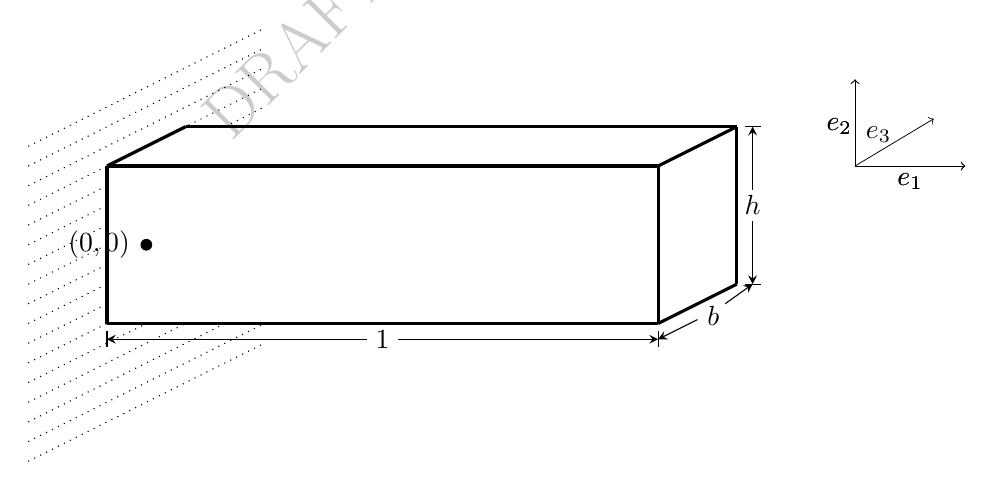
\begin{tikzpicture}
		
		\draw[line width = 0.4mm] (-0.5,1) -- (6.5,1);
		\draw[line width = 0.4mm] (-0.5,-1) -- (6.5,-1);
		\draw[line width = 0.4mm] (6.5,-1) -- (6.5,1);
		\draw[line width = 0.4mm] (-0.5,-1) -- (-0.5,1);
		
		\draw[line width = 0.4mm] (0.5,1.5) -- (7.5,1.5);
		\draw[line width = 0.4mm] (7.5,-0.5) -- (7.5,1.5);
		
		
		\draw[line width = 0.4mm] (-0.5,1) -- (0.5,1.5);
		\draw[line width = 0.4mm] (6.5,1) -- (7.5,1.5);
		\draw[line width = 0.4mm] (6.5,-1) -- (7.5,-0.5);
		
		
		
		\draw[scale=0.5, domain=-3:3, smooth, variable=\x,dotted] plot ({\x}, {0.5*\x+4});
		\draw[scale=0.5, domain=-3:3, smooth, variable=\x,dotted] plot ({\x}, {0.5*\x+3.5});
		\draw[scale=0.5, domain=-3:3, smooth, variable=\x,dotted] plot ({\x}, {0.5*\x+3});
		\draw[scale=0.5, domain=-3:3, smooth, variable=\x,dotted] plot ({\x}, {0.5*\x+2.5});
		
		\draw[scale=0.5, domain=-3:-1, smooth, variable=\x,dotted] plot ({\x}, {0.5*\x+2});
		\draw[scale=0.5, domain=2:3, smooth, variable=\x,dotted] plot ({\x}, {0.5*\x+2});
		
		\draw[scale=0.5, domain=-3:-1, smooth, variable=\x,dotted] plot ({\x}, {0.5*\x+1.5});
		\draw[scale=0.5, domain=-3:-1, smooth, variable=\x,dotted] plot ({\x}, {0.5*\x+1});
		\draw[scale=0.5, domain=-3:-1, smooth, variable=\x,dotted] plot ({\x}, {0.5*\x+0.5});
		\draw[scale=0.5, domain=-3:-1, smooth, variable=\x,dotted] plot ({\x}, {0.5*\x});
		\draw[scale=0.5, domain=-3:-1, smooth, variable=\x,dotted] plot ({\x}, {0.5*\x-0.5});
		\draw[scale=0.5, domain=-3:-1, smooth, variable=\x,dotted] plot ({\x}, {0.5*\x-1});
		\draw[scale=0.5, domain=-3:-1, smooth, variable=\x,dotted] plot ({\x}, {0.5*\x-1.5});
		\draw[scale=0.5, domain=-3:0, smooth, variable=\x,dotted] plot ({\x}, {0.5*\x-2});
		\draw[scale=0.5, domain=-3:1, smooth, variable=\x,dotted] plot ({\x}, {0.5*\x-2.5});
		\draw[scale=0.5, domain=-3:2, smooth, variable=\x,dotted] plot ({\x}, {0.5*\x-3});
		\draw[scale=0.5, domain=-3:3, smooth, variable=\x,dotted] plot ({\x}, {0.5*\x-3.5});
		\draw[scale=0.5, domain=-3:3, smooth, variable=\x,dotted] plot ({\x}, {0.5*\x-4});
		
		%\node at (6.9,1) {$b$};
		%\node at (6.65,0) {$h$};
		%\node at (3.2,-1.2) {$\ell = 1$};
		
		\draw[line width = 0.1mm,->] (9,1) -- (10,1.6);
		\draw[line width = 0.1mm,->] (9,1) -- (10.4,1);
		\draw[line width = 0.1mm,->] (9,1) -- (9,2.1);
		\node at (9.3,1.4) {$e_3$};
		\node at (9.7,0.8) {$e_1$};
		\node at (8.8,1.5) {$e_2$};
		
		\node at (7.7,0.5) {$h$};
		\draw[-stealth] (7.7,0.7) -- (7.7,1.5);
		\draw (7.6,1.5) -- (7.8,1.5);
		\draw[-stealth] (7.7,0.3) -- (7.7,-0.5);
		\draw (7.6,-0.5) -- (7.8,-0.5);
		
		\node at (3,-1.2) {$1$};
		\draw[stealth-] (-0.5,-1.2) -- (2.8,-1.2);
		\draw[stealth-] (6.5,-1.2) -- (3.2,-1.2);
		\draw (6.5,-1.3) -- (6.5,-1.1);
		\draw (-0.5,-1.3) -- (-0.5,-1.1);
		
		\node at (7.2,-0.9) {$b$};
		\draw[stealth-] (7.7,-0.5) -- (7.35,-0.75);
		\draw[stealth-] (6.5,-1.2) -- (7,-0.95);
		
		\draw[line width = 0.1mm,->] (9,1) -- (10.4,1);
		\draw[line width = 0.1mm,->] (9,1) -- (9,2.1);
		\node at (9.7,0.8) {$e_1$};
		\node at (8.8,1.5) {$e_2$};
		
		\node at (-0.6,0) {$(0,0)$};
		\node at (0,0)[circle,fill,inner sep=1.5pt]{};
		
		%\node at (-1.4,-1.3) {$(0,-\frac{h}{2},-\frac{b}{2})$};
		%\node at (-1.4,1) {$(0,\frac{h}{2},-\frac{b}{2})$};
		%\node at (0.5,1.8) {$(0,\frac{h}{2},\frac{b}{2})$};
		
		%\node at (6,-1.3) {$(1,-\frac{h}{2},-\frac{b}{2})$};
		%\node at (6.3,0.7) {$(1,\frac{h}{2},-\frac{b}{2})$};
		%\node at (7.5,1.8) {$(1,\frac{h}{2},\frac{b}{2})$};
		%\node at (8.4,-0.4) {$(1,-\frac{h}{2},\frac{b}{2})$};
		
	\end{tikzpicture}
	
\end{figure} 


In Section \ref{ssec:3D_Model:VariationalForm}, the variational problem for the three-dimensional cantilever model is defined by Problem 3DV. This general form can now be rewritten as in a model specific form using the reference configuration. For convenience, some of the results from Section \ref{sec:3D_Model} are repeated here.

\subsubsection{Problem 3DV}
Find a function $u$ such that for all $t>0$, $u \in T(\Omega)$ and 
\begin{align}
	c(u,\phi) = -b(u,\phi) - (Q,\phi) \label{3DB_20}
\end{align}
for all $\phi \in T(\Omega)$.\\

With the test function space
\begin{eqnarray*}
	T(\Omega) & = & \left\{ \phi \in C(\Omega) \ | \ \phi = 0 \ \textrm{ on } \ \Gamma \right\}.
\end{eqnarray*}

The bilinear forms and integral function are defined by
\begin{eqnarray}
	b(u,\phi) &=& \int_\Omega~c_1\textrm{Tr}({\cal E}\Phi)+ c_2\textrm{Tr}({\cal E})
	\textrm{Tr}(\Phi) ~dV,\\
	c(u,\phi) &=& \int_\Omega~ (\partial^2_t u) \cdot \phi~dV, \\
	(f,g) &=& \int_{\Omega} f\cdot g \ dV, \\
\end{eqnarray}
with $\displaystyle c_1 = \frac{1}{\gamma(1+\nu)}$ and $\displaystyle c_2 = \frac{\nu}{\gamma(1+\nu)(1-2\nu)}$.\\

Using the definition of the reference configuration, the constitutive equations and the bilinear form $b$ can be rewritten in the following model specific forms: 
\subsubsection*{Constitutive equations}
\begin{eqnarray*}
	\sigma_{11} & = &  \frac{1}{\gamma(1+\nu)}\partial_1 u_1 + \frac{\nu}{\gamma (1+\nu)(1-2\nu)}(\partial_1 u_1 +  \partial_2 u_2 + \partial_3 u_3)\label{3DB_3}\\
	\sigma_{22} & = &  \frac{1}{\gamma(1+\nu)}\partial_2 u_2 + \frac{\nu}{\gamma (1+\nu)(1-2\nu)}(\partial_1 u_1 +  \partial_2 u_2 + \partial_3 u_3)\label{3DB_4}\\
	\sigma_{33} & = &  \frac{1}{\gamma(1+\nu)}\partial_3 u_3 + \frac{\nu}{\gamma (1+\nu)(1-2\nu)}(\partial_1 u_1 +  \partial_2 u_2 + \partial_3 u_3)\label{3DB_5}\\
	\sigma_{23} & = &  \frac{1}{2\gamma(1+\nu)}(\partial_3 u_2 + \partial_2 u_3)\label{3DB_6}\\
	\sigma_{31} & = &  \frac{1}{2\gamma(1+\nu)}(\partial_3 u_1 + \partial_1 u_3)\label{3DB_7}\\
	\sigma_{12} & = &  \frac{1}{2\gamma(1+\nu)}(\partial_2 u_1 + \partial_1 u_2)\label{3DB_8}
\end{eqnarray*}

\subsubsection{Bilinear Form}
\begin{align*}
	b(u,\phi)  &=  \int_\Omega~c_1\textrm{Tr}({\cal E}\Phi)+ c_2\textrm{Tr}({\cal E})
	\textrm{Tr}(\Phi) ~dV \nonumber\\
	 &=  \int_{\Omega} \sigma_{11} \partial_1\phi_1 + \sigma_{12}\partial_1 \phi_2 + \sigma_{13}\partial_1 \phi_3 + \sigma_{21}\partial_2 \phi_1 + \sigma_{22}\partial_2\phi_2 + \sigma_{23}\partial_2 \phi_3 ~dV
\end{align*}

\subsection{Weak variational form}

\subsubsection{Bilinear form}
Define the inertia space $V$ as the closure of $T(\Omega)$ in $H := H^1(0,1)\times H^1(0,1)\times H^1(0,1)$. Denote $X = L^2(0,1)\times L^2(0,1)\times L^2(0,1)$. The inertia space is $W  = X$ with norm $||\cdot||_W = \sqrt{c(\cdot,\cdot)}$.

\subsubsection{Problem 3DW}
Find a function $u$ such that for all $t>0$, $u(t) \in V$ and $u''(t) \in W$, satisfying the following equation
\begin{eqnarray}
	c(u,v) + b(u,v) & = & (Q,v) \ \ \ \textrm{ for each } v \in V.
\end{eqnarray}

\subsection{Galerkin approximation}
As mentioned in the previous section, Section \ref{2d_FEM_G}, the body $\Omega$ needs to be descritised. For this is three-dimensional body, three-dimensional elements shapes are required. The elements used in this dissertation are rectangular prismatic elements. These elements are also known as `brick-shaped' elements and is described in \cite{Wu06}. This shape of element is a natural choice for a three-dimensional elastic body with a rectangular cross-section.

Divide the reference configuration $\Omega$ into a grid of rectangular prismatic elements, such that there are $n = n_1 \times n_2 \times n_3$ nodes.

Define a set of $n$-dimensional linear independent basis functions. For the three-dimensional model, the basis functions can be defined by the set
\begin{eqnarray*}
 B = \{\langle\phi_1, 0 , 0\rangle, \langle\phi_2, 0, 0\rangle,...,\langle\phi_{n}, 0, 0 \rangle,\\
	\langle 0,\phi_1 ,0 \rangle,\langle 0 ,\phi_2,0\rangle,...,\langle 0,\phi_{n},0\rangle,\\
	\langle 0,0,\phi_1 \rangle,\langle 0,0,\phi_2\rangle,...,\langle 0,0,\phi_{n}\rangle \}.
\end{eqnarray*}

For the this three-dimensional model, piecewise Hermite tri-cubic basis functions are used. Although this is more complex than using piecwise tri-linear basis functions, as mentioned in Section \ref{2d_FEM_G}, the tri-cubic basis functions ensure faster convergence and also the derivatives of the solutions.

Recall that the admissible basis functions, are all the basis functions that satisfies all the conditions of the test function space $T(\Omega)$. Denote the admissible basis functions by $\delta_j$, with each $\delta_j$ a unique element of $B$. The set of admissible basis functions can then be expressed as $A = \left\{\delta_1, \delta_2,... , \delta_k\right\}$ with $k \leq 3n$.

Define the space
\begin{eqnarray*}
	S^h & = & \textrm{span}\left(\left\{\delta_i \ | \ i = 1,2,...,k \right\} \right)
\end{eqnarray*}

For each function $u^h \in S^h$, $u^h$ can be expressed as
\begin{eqnarray*}
	u^h = \sum_{i = 1}^{k} u_i(t) \delta_{i}(x)
\end{eqnarray*}

Substituting $u^h$ into Problem 3DV, results in the following Galerkin approximation, denoted by Problem 3DG.

\subsubsection{Problem 3DG}
Find a function $u^h$ such that for all $t>0$, $u^h \in S^h$ and
\begin{eqnarray*}
	(u^h, \phi_i) & = & -b(u^h,\phi_i) + (Q^I \cdot \phi_i)
\end{eqnarray*} for $i = 1,2,...,k$. $Q^I$ is scalar vector obtained after interpolating the function $Q$ over the rectangular grid $\Omega$. i.e. $Q^I_{i,j, h} = Q(x_i,x_j, x_h)$ for $i = 1,2,...,n_1$, $j = 1,2,...,n_2$ and $h = 1,2,...,n_3$.

\subsection{System of ordinary differential equations}\label{3d_fem_g}
Consider the following standard Finite Element Method matrices.

\subsubsection{FEM matrices}
\noindent\begin{minipage}{.5\linewidth}
	\begin{eqnarray*}
		\mathbf{M}_{ij} & = & \int_{\Omega} \phi_j \phi_i \ dV \ \\
		{K_{11}}_{ij} & = & \int_{\Omega} \partial_1\phi_j \partial_1\phi_i \ dV \  \\
		{K_{12}}_{ij} & = & \int_{\Omega} \partial_1\phi_j \partial_2\phi_i \ dV \ \\
		{K_{13}}_{ij} & = & \int_{\Omega} \partial_1\phi_j \partial_3\phi_i \ dV \ 
	\end{eqnarray*}
\end{minipage}%
\begin{minipage}{.5\linewidth}
	\begin{eqnarray*}
		{K_{22}}_{ij} & = & \int_{\Omega} \partial_2\phi_j \partial_2\phi_i \ dV \  \\
		{K_{23}}_{ij} & = & \int_{\Omega} \partial_2\phi_j \partial_3\phi_i \ dV \ \\
		{K_{33}}_{ij} & = & \int_{\Omega} \partial_3\phi_j \partial_3\phi_i \ dV \ \\
	\end{eqnarray*}
\end{minipage}
for $i,j = 1,2,...,k.$\\

And

\begin{eqnarray*}
	\mathbf{M_f}_{ij} & = & \int_{\Omega} \phi_j \phi_i \ dV
\end{eqnarray*}
for $i = 1,2,...,k$ and for $j = 1,2,...,3n.$\\

The remaining matrices can be defined as
\begin{eqnarray*}
	{K_{21}} & = & {K_{12}}^{T},\\
	{K_{31}} & = & {K_{13}}^{T}, \\
	{K_{32}} & = & {K_{23}}^{T}. \\
\end{eqnarray*}

Define the following matrices:\\
\noindent\begin{minipage}{.5\linewidth}
	\begin{eqnarray*}
		\mathbf{K11} & = & \left(C_1 + C_2 \right) K_{11} + C_3 K_{22} + C_3 K_{33}\\
		\mathbf{K12} & = & C_3 K_{12} + C_2 K_{21}\\
		\mathbf{K13} & = & C_3 K_{13} + C_2 K_{31}\\
		\mathbf{K21} & = & C_3 K_{21} + C_2 K_{12}\\
		\mathbf{K22} & = & \left(C_1 + C_2 \right) K_{22} + C_3 K_{11} + C_3 K_{33}
	\end{eqnarray*}
\end{minipage}%
\begin{minipage}{0.8\linewidth}
	\begin{eqnarray*}
		\mathbf{K23} & = & C_3 K_{23} + C_2 K_{32}\\
		\mathbf{K31} & = & C_3 K_{31} + C_2 K_{13}\\
		\mathbf{K32} & = & C_3 K_{32} + C_2 K_{23}\\
		\mathbf{K33} & = & \left(C_1 + C_3 \right) K_{33} + C_3 K_{11} + C_3 K_{22}
	\end{eqnarray*}
\end{minipage}\\

with $C_1 = \frac{1}{\gamma(1+\nu)}$, $C_2 =  \frac{\nu}{\gamma (1+\nu)(1-2\nu)}$ and $C_3 =  \frac{1}{2\gamma(1-2\nu)}$.\\

Using the standard FEM matrices and the matrices $K11$ to $K33$, the following concatenated matrices are defined:\\


\begin{eqnarray}
	\begin{aligned}
		K = 
		\begin{bmatrix}
			\mathbf{K11} & \mathbf{K12} & \mathbf{K13}\\
			\mathbf{K21} & \mathbf{K22} & \mathbf{K23}\\
			\mathbf{K31} & \mathbf{K32} & \mathbf{K33}
		\end{bmatrix}
	\end{aligned}
	\ \ \ \ \ \ \ \ \
	\begin{aligned}
		M  = 
		\begin{bmatrix}
			\mathbf{M} & {O} & {O}\\
			{O} & \mathbf{M} & {O}\\
			{O} & {O} & \mathbf{M}
		\end{bmatrix}
	\end{aligned}\label{eq:3DFEM:K+M}
\end{eqnarray}



\begin{eqnarray}
	M_f & = &
	\begin{bmatrix}
		\mathbf{M_f} & {O_f} & {O_f}\\
		{O_f} & \mathbf{M_f} & {O_f}\\
		{O_f} & {O_f} & \mathbf{M_f}
	\end{bmatrix}\label{eq:3DFEM:M}
\end{eqnarray}
The matrices ${O}$ and ${O_f}$ are the zero matrices of the same size as $\mathbf{M}$ and $\mathbf{M_f}$ respectively.\\

Using \eqref{eq:3DFEM:K+M} and \eqref{eq:3DFEM:M}, Problem 3DG is rewritten as a system of ordinary differential equations. This system is referred to as Problem 3DODE

\subsubsection{Problem 3DODE}
Find a function $\bar{u} \in S^h$ such that
\begin{eqnarray}
	M\ddot{\bar{u}} & = & K\bar{u} + M_{f}Q^I. \label{3D_M}
\end{eqnarray} With $\bar{u}$ in the form $\bar{u} = \partial^i_1u \partial^j_2u \partial^k_3u$ for $i,j,k = 0,1,2,3$.

\subsection{Eigenvalue problem}
The derivation and form of the eigenvalue problem for the three-dimensional elastic body is similar to the two-dimensional model given in Section \ref{2dFEM_EP}.

\subsubsection{Problem 3DE}\label{3dFEM_EP}
Find a real number $\lambda$ and a function $\bar{u} \in S^h$ such that
\begin{eqnarray}
	M\lambda{\bar{u}} & = & K\bar{u}.
\end{eqnarray}


Consider a cantilever two-dimensional elastic body, with a rectangular cross-section.

\subsubsection{Reference configuration for rectangular cross-section}\label{sssec:2D_Model:RefConf}
Let $\{e_1,e_2\}$ be a right-handed orthonormal basis for $R^2$. Denote the elastic body by $\Omega \in R^2$, with $(0,0)$ as the point of reference. For a rectangular cross-section, the body $\Omega$ can be described as,
\begin{eqnarray*}
	\Omega = \left \{ x \in E_2 \ | \ 0 \leq x_1 \leq 1, \ -\frac{h}{2} \leq x_2 \leq \frac{h}{2} \right \},
\end{eqnarray*} where $\partial \Omega$ denotes the boundary of $\Omega$. The boundary $\partial \Omega$ can be divided into the four distinct lines (or edges) as follows: \label{sym:En}

\noindent\begin{minipage}{.5\linewidth}
	\begin{eqnarray*}
		\Sigma:& \quad x_1 &= 0\\
		\Gamma_3:& \quad x_1 &= 1
	\end{eqnarray*}
\end{minipage}%
\begin{minipage}{.5\linewidth}
	\begin{eqnarray*}
		\Gamma_1:& \quad x_2 &= -{h}/{2}\\
		\Gamma_2:& \quad x_2 &= {h}/{2}
	\end{eqnarray*}
\end{minipage}

In this configuration, the body is clamped rigidly to the surface at $x_1 = 0$ denoted as $\Sigma$ and the body is free-hanging on the other boundaries denoted by $\Gamma$.

\subsubsection{Cantilever elastic body}
Consider a two-dimensional elastic body clamped rigidly to a surface at $x_1 = 0$. The body is free-hanging on the other boundaries. This is Problem 2D in Section \ref{ssec:2D_Model:ModelProblem}.

\begin{figure}[h!]
	\centering
	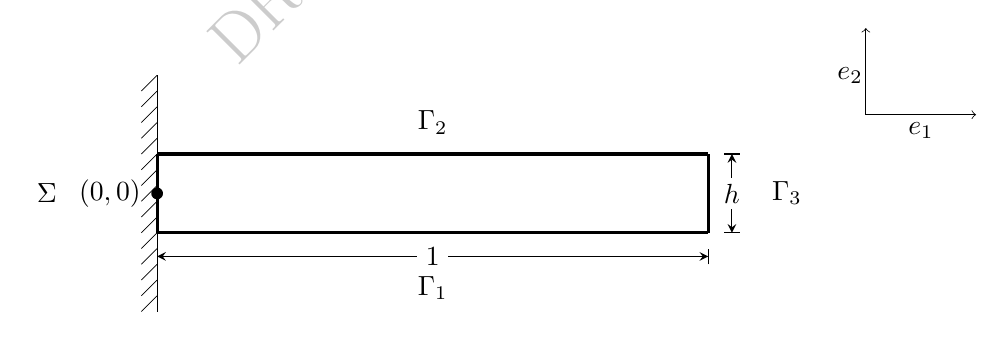
\begin{tikzpicture}
		
		\draw[line width = 0.4mm] (0,0.5) -- (7,0.5);
		\draw[line width = 0.4mm] (0,-0.5) -- (7,-0.5);
		\draw[line width = 0.4mm] (7,-0.5) -- (7,0.5);
		\draw[line width = 0.4mm] (0,-0.5) -- (0,0.5);
		
		\draw[line width = 0.1mm] (0,1.5) -- (0,-1.5);
		
		\draw[line width = 0.1mm] (0,1.5) -- (-0.2,1.3);
		\draw[line width = 0.1mm] (0,1.3) -- (-0.2,1.1);
		\draw[line width = 0.1mm] (0,1.1) -- (-0.2,0.9);
		\draw[line width = 0.1mm] (0,0.9) -- (-0.2,0.7);
		\draw[line width = 0.1mm] (0,0.7) -- (-0.2,0.5);
		\draw[line width = 0.1mm] (0,0.5) -- (-0.2,0.3);
		\draw[line width = 0.1mm] (0,0.3) -- (-0.2,0.1);
		\draw[line width = 0.1mm] (0,0.1) -- (-0.2,-0.1);
		\draw[line width = 0.1mm] (0,-0.1) -- (-0.2,-0.3);
		\draw[line width = 0.1mm] (0,-0.3) -- (-0.2,-0.5);
		\draw[line width = 0.1mm] (0,-0.5) -- (-0.2,-0.7);
		\draw[line width = 0.1mm] (0,-0.7) -- (-0.2,-0.9);
		\draw[line width = 0.1mm] (0,-0.9) -- (-0.2,-1.1);
		\draw[line width = 0.1mm] (0,-1.1) -- (-0.2,-1.3);
		\draw[line width = 0.1mm] (0,-1.3) -- (-0.2,-1.5);
		
		\node at (7.3,0) {$h$};
		\draw[-stealth] (7.3,0.2) -- (7.3,0.5);
		\draw (7.2,0.5) -- (7.4,0.5);
		\draw[-stealth] (7.3,-0.2) -- (7.3,-0.5);
		\draw (7.2,-0.5) -- (7.4,-0.5);
		
		\node at (3.5,-0.8) {$1$};
		\draw[stealth-] (0,-0.8) -- (3.3,-0.8);
		\draw[stealth-] (7,-0.8) -- (3.7,-0.8);
		\draw (7,-0.9) -- (7,-0.7);
		
		\draw[line width = 0.1mm,->] (9,1) -- (10.4,1);
		\draw[line width = 0.1mm,->] (9,1) -- (9,2.1);
		\node at (9.7,0.8) {$e_1$};
		\node at (8.8,1.5) {$e_2$};
		
		\node at (-0.6,0) {$(0,0)$};
		\node at (0,0)[circle,fill,inner sep=1.5pt]{};

		% Add Σ at x_1 = 0
		\node at (-1.4,0) {$\Sigma$};
		
		% Add Γ₁ at x_2 = -h/2
		\node at (3.5,-1.2) {$\Gamma_1$};
		
		% Add Γ₂ at x_2 = h/2
		\node at (3.5,0.9) {$\Gamma_2$};
		
		% Add Γ₃ at x_1 = 1
		\node at (8,0) {$\Gamma_3$};
		
	\end{tikzpicture}
\end{figure} 


In Section \ref{ssec:2D_Model:VariationalForm} the variational problem for the two dimensional cantilever model is derived and refered to as Problem 2DV. Some of the results from Section \ref{sec:2D_Model} are repeated here for convenience. Using the reference configuration, these results are rewritten from a general form to a model specific form.

\subsubsection{Problem 2DV}\label{sssec:2D_Model:Problem2D1VChp5}
Find a function $u$ such that for all $t>0$, $u \in T(\Omega)$ and 
\begin{align}
	c(u,\phi) = -b(u,\phi) + (Q,\phi) \label{eq:2D_Model:Problem2D1VEqChp5}
\end{align}
for all $\phi \in T(\Omega)$. With the test function space 
\begin{eqnarray*}
	T(\Omega) & = & \left\{ \phi \in C^1(\bar{\Omega}) \ | \ \phi = 0 \ \textrm{ on } \ \Gamma \right\}.
\end{eqnarray*}

The bilinear forms and integral function is defined by
\begin{eqnarray}
	b(u,\phi) & = & \int_\Omega~c_1\textrm{Tr}({\cal E}\Phi)+ c_2\textrm{Tr}({\cal E})
	\textrm{Tr}(\Phi) ~dA, \label{eq:2D_Model:BilinearChp5}\\
	c(\partial_t^2 u,\phi) & = & \int_\Omega~ (\partial^2_t u) \cdot \phi~dA, \label{eq:2D_Model:Bilinear_cChp5}\\
	(f,g) &=& \int_{\Omega} f\cdot g \ dA, \label{eq:2D_Model:Bilinear_intChp5}
\end{eqnarray}
with $\displaystyle c_1 = \frac{1}{\gamma(1+\nu)}$ and $\displaystyle c_2 = \frac{\nu}{\gamma(1-\nu^2)}$.

Using the reference configuration, the constitutive equations and the bilinear form $b$ can be rewritten into a model specific form.

\subsubsection{Constitutive equations:}
\begin{eqnarray}
	\sigma_{11} & = & \frac{1}{\gamma(1-\nu^2)}(\partial_1 u_1 + \nu \partial_2 u_2) \label{CE1} \\
	\sigma_{22} & = & \frac{1}{\gamma(1-\nu^2)}(\partial_2 u_2 + \nu \partial_1 u_1) \label{CE2} \\
	\sigma_{12} & = & \frac{1}{2\gamma(1+\nu)}(\partial_1 u_2 + \partial_2 u_1) \label{CE3}
\end{eqnarray}

\subsubsection{Bilinear form:}
\begin{align}
	b(u,\phi) & = & \frac{1}{\gamma(1-\nu^2)}\int_{\Omega} (\partial_1 u_1 \partial_1 \phi_1 + \partial_2 u_2 \partial _2 \phi_2 + \nu\partial_1 u_1 \partial_2\phi_2 + \nu \partial_2 u_2 \partial_1 \phi_1 ) \ dA \nonumber\\
	& + & \frac{1}{2\gamma(1+\nu)}\int_{\Omega} (\partial_1 u_2 \partial_1 \phi_2 + \partial_1 u_2 \partial_2 \phi_1 + \partial_2 u_1 \partial_1\phi_2 + \partial_2 u_1 \partial_2\phi_1) \ dA.
\end{align}

\subsection{Weak variational form}
Define the inertia space $V$ as the closure of $T(\Omega)$ in $H := H^1(0,1)\times H^1(0,1)$. Denote $X = L^2(0,1)\times L^2(0,1)$. The inertia space is $W  = X$ with norm $||\cdot||_W = \sqrt{c(\cdot,\cdot)}$.

\subsubsection{Problem 2DWV}
Find a function $u$ such that $\forall \ t > 0$, $u \in V$ with $\partial_t^2 u \in W$ and
\begin{eqnarray*}
	c(u,v) + b(u,v) & = & (Q,v)
\end{eqnarray*}
for all $v\in V$.


\subsection{Galerkin approximation}\label{2d_FEM_G}
To be able to apply the Finite Element Method to Problem 2DV, the body $\Omega$ needs to be discretised. This is done by dividing the body $\Omega$ into discrete shapes, called elements. There are various types of shapes of elements that can be used. Since the body $\omega$ is has a rectangular cross-section, rectangular elements are the simplest elements to use.

Divide the reference configuration $\Omega$ into a grid of rectangular elements, such that there are $n = n_1\times n_2$ nodes.

Define a set of $n$-dimensional linear independent basis functions. For the two dimensional model, the basis functions can be defined by the set $$B = \left\{\langle\phi_1, 0\rangle, \langle\phi_2, 0\rangle,...,\langle\phi_{n}, 0 \rangle,\langle 0,\phi_1\rangle,\langle 0 ,\phi_2\rangle,...,\langle 0,\phi_{n}\rangle \right\}.$$ 

These functions are chosen as piecewise Hermite bi-cubic functions $\phi_i$. Simpler bi-linear functions can also be used, however the use of the bi-cubic basis functions results in faster convergence and also the benefit of obtaining the derivatives of the solution at the expense of more complexity.

The subset of basis functions $B$ that satisfies all the conditions of the test function space $T(\Omega)$ are called the admissible basis functions. Denote the admissible basis functions by $\delta_j$, where each $\delta_j$ is a unique element of $B$. The admissible basis functions can be numbered and expressed as the set $A = \left \{\delta_1, \delta_2,..., \delta_k \right\}$ for some $k \leq 2n$.\\ 

Define the space
\begin{eqnarray*}
S^h & = & \textrm{span}\left(\left\{\delta_i \ | \ i = 1,2,...,k \right\} \right).
\end{eqnarray*}

For each function $u^h \in S^h$, $u^h$ can be expressed as
\begin{eqnarray*}
	u^h = \sum_{i = 1}^{k} u_i(t) \delta_{i}(x).
\end{eqnarray*}

Substitution of $u^h$ into Problem 2DV, results in the following Galerkin Approximation, denoted by Problem 2DG.

\subsubsection{Problem 2DG}
Find a function $u^h$ such that for all $t>0$, $u^h \in S^h$ and
\begin{eqnarray*}
	(u^h, \phi_i) & = & -b(u^h,\phi_i) + (Q^I, \phi_i)
\end{eqnarray*} for $i = 1,2,...,k$. $Q^I$ is scalar vector obtained after interpolating the function $Q$ over the rectangular grid $\Omega$. i.e. $Q^I_{i,j} = Q(x_i,x_j)$ for $i = 1,2,...,n_1$ and $j = 1,2,...,n_2$.

\subsection{System of differential equations}\label{ssec:2DFEM:DE}

Consider the following standard Finite Element Method matrices
\subsubsection{FEM matrices}
\noindent\begin{minipage}{.5\linewidth}
	\begin{eqnarray*}
		\mathbf{M}_{j,i} & = & \int_{\Omega} \phi_i \phi_j ~dA \\
		\mathbf{{K}_{11}}_{j,i} & = & \int_{\Omega} \partial_1\phi_i \partial_1\phi_j~dA\\
		\mathbf{{K}_{22}}_{j,i} & = & \int_{\Omega} \partial_2\phi_i \partial_2\phi_j~dA
	\end{eqnarray*}
\end{minipage}%
\begin{minipage}{.5\linewidth}
	\begin{eqnarray*}
		\mathbf{{K}_{12}}_{j,i} & = & \int_{\Omega} \partial_2\phi_i \partial_1\phi_j~dA\\
		\mathbf{{K}_{21}}_{j,i} & = & \int_{\Omega} \partial_1\phi_i \partial_2\phi_j~dA
	\end{eqnarray*}
\end{minipage}
for $i,j = 1,2,...,k$.

And 
\begin{eqnarray*}
	{M_{F}}_{j,i} = \int_{\Omega}  \phi_i \phi_j~dA
\end{eqnarray*}

for $i = 1,2,...,k$ and for $j =1,2,...,2n$.

Define the following matrices:
\begin{eqnarray*}
	K_1 & = & \frac{1}{\gamma(1-\nu^2)} \mathbf{K_{11}} + \frac{1}{2\gamma(1+\nu)}\mathbf{K_{22}} \label{eq:2DFEM:K1} \\
	K_2 & = & \frac{\nu}{\gamma(1-\nu^2)} \mathbf{K_{21}} + \frac{1}{2\gamma(1+\nu)}\mathbf{K_{12}}\label{eq:2DFEM:K2}\\
	K_3 & = & \frac{\nu}{\gamma(1-\nu^2)} \mathbf{K_{12}} + \frac{1}{2\gamma(1+\nu)}\mathbf{K_{21}}\label{eq:2DFEM:K3}\\
	K_4 & = & \frac{1}{\gamma(1-\nu^2)} \mathbf{K_{22}} + \frac{1}{2\gamma(1+\nu)}\mathbf{K_{11}}\label{eq:2DFEM:K4}
\end{eqnarray*}

Using the standard FEM matrices and matrices $K_1$-$K_4$, the following concatenated matrices are defined.
\begin{eqnarray}
	\begin{aligned}
		K = 
		\begin{bmatrix}
			K1 & K2\\
			K3 & K4
		\end{bmatrix}
	\end{aligned}
	\ \ \ \ \ \ \ \ \
	\begin{aligned}
		M_f = 
		\begin{bmatrix}
			M_{F} & O_{F}\\
			O_{F} & M_{F}
		\end{bmatrix}
	\end{aligned}\label{eq:2DFEM:K+M}
\end{eqnarray}

\begin{eqnarray}
	M = 
	\begin{bmatrix}
		\mathbf{M} & O \\
		O & \mathbf{M}
	\end{bmatrix}\label{eq:2DFEM:M}
\end{eqnarray}

The matrices ${O}$ and ${O_f}$ are the zero matrices of the same size as $\mathbf{M}$ and ${M_f}$ respectively.

Using \eqref{eq:2DFEM:K+M} and \eqref{eq:2DFEM:M}, Problem 2DG is rewritten as a system of ordinary differential equations. This system is referred to as Problem 2DODE.

\subsubsection{Problem 2DODE}
Find a function $\bar{u} \in S^h$ such that
\begin{eqnarray}
	M\ddot{\bar{u}} & = & K\bar{u} + M_{f}Q^I.
\end{eqnarray} With $\bar{u}$ in the form $\bar{u} = \langle u, \partial_1 u, \partial_2 u, \partial_{12} u \rangle$.

\textbf{Remark} This form of $\bar{u}$ is determined by the use of the bi-cubic basis functions.

\subsection{Eigenvalue problem}\label{2dFEM_EP}
For the eigenvalue problem, assume that there is no external force, $M_{f}Q^I = 0$, so that 
\begin{eqnarray}
		M\ddot{\bar{u}} & = & K\bar{u}.\label{eq:2DFEM:M2}
\end{eqnarray}
It is known that a system of ordinary differential equations has a general solution of the form $e^{rt}$. Suppose that $\bar{w} = e^{\lambda t} \bar{u}$ is a solution for \eqref{eq:2DFEM:M2}. In this solution, $\lambda$ is an eigenvalue and $\bar{u}$ a corresponding eigenfunction. Substitution into \eqref{eq:2DFEM:M2} results in
\begin{eqnarray*}
	M\lambda e^{\lambda t}\bar{u} & = & Ke^{\lambda t}\bar{u}.
\end{eqnarray*}
Since $e^{\lambda t} > 0$ for all values of $\lambda t$, we can cancel it from both sides of the equation and formulate the eigenvalue problem Problem 2DE.

\subsubsection{Problem 2DE}
Find a real number $\lambda$ and a function $\bar{u} \in S^h$ such that
\begin{eqnarray}
	M\lambda{\bar{u}} & = & K\bar{u}.
\end{eqnarray}



\section{Results}

\section{Validity of a model for a cantilever two-dimensional beam} \label{sec:validity-of-a-2d-beam}

In Section \ref{sec:validity-of-a-cantilever-timoshenko-beam}, the article \cite{LVV09} was discussed. In this article, the authors investigated the validity of a cantilever Timoshenko beam by comparing it to a cantilever two-dimensional beam. In this section, the article is extended and the validity of the cantilever two-dimensional model is investigated.

As mentioned in the introduction of the chapter, a beam is a three-dimensional body and therefore a three-dimensional model is more realistic. However the authors of \cite{LVV09} mention that a direct comparison of the one and three-dimensional models will have complexities and they suggest using the two-dimensional model as an intermediate step.

So in this section, the article \cite{LVV09} is extended and the validity of a cantilever two-dimensional beam model is investigated, using a cantilever three-dimensional model as a reference.

\subsection{The models}
The two-dimensional model is the same model as used in the previous section, Problem T-2 defined in Section \ref{ssec:2D_Model:ModelProblem}. From Section \ref{ssec:3D_Model:ModelProblems}, the cantilever three-dimensional model, referred to as Problem 3D.

Figure \ref{fig:2Dv3D} shows the two beams side-by-side.

\begin{figure}[h!]
	\scalebox{.8}{
		\makebox[\textwidth][c]{

			\centering
			\begin{minipage}[b]{0.7\linewidth}
				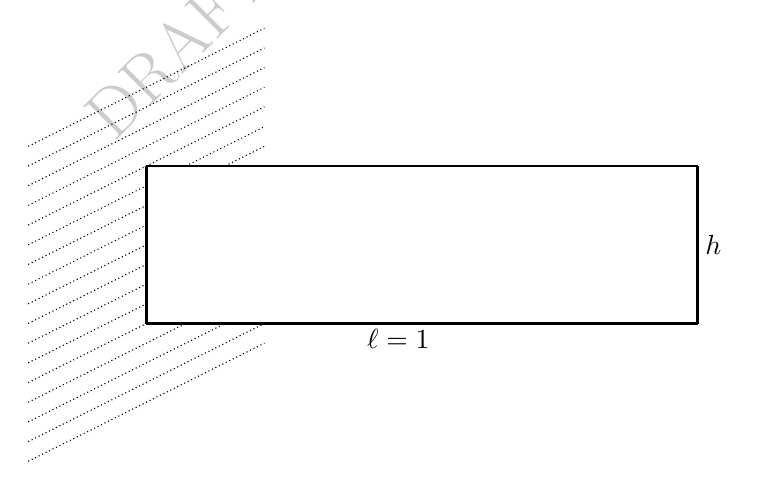
\begin{tikzpicture}
					\draw[line width = 0.3mm] (0,1) -- (7,1);
					\draw[line width = 0.3mm] (0,-1) -- (7,-1);
					\draw[line width = 0.3mm] (7,-1) -- (7,1);
					\draw[line width = 0.3mm] (0,-1) -- (0,1);
					
					
					\draw[scale=0.5, domain=-3:3, smooth, variable=\x,densely dotted] plot ({\x}, {0.5*\x+4});
					\draw[scale=0.5, domain=-3:3, smooth, variable=\x,densely dotted] plot ({\x}, {0.5*\x+3.5});
					\draw[scale=0.5, domain=-3:3, smooth, variable=\x,densely dotted] plot ({\x}, {0.5*\x+3});
					\draw[scale=0.5, domain=-3:3, smooth, variable=\x,densely dotted] plot ({\x}, {0.5*\x+2.5});
					\draw[scale=0.5, domain=-3:3, smooth, variable=\x,densely dotted] plot ({\x}, {0.5*\x+2});
					
					\draw[scale=0.5, domain=-3:0, smooth, variable=\x,densely dotted] plot ({\x}, {0.5*\x+1.5});
					\draw[scale=0.5, domain=-3:0, smooth, variable=\x,densely dotted] plot ({\x}, {0.5*\x+1});
					
					
					\draw[scale=0.5, domain=1:3, smooth, variable=\x,densely dotted] plot ({\x}, {0.5*\x+1.5});
					\draw[scale=0.5, domain=2:3, smooth, variable=\x,densely dotted] plot ({\x}, {0.5*\x+1});
					
					\draw[scale=0.5, domain=-3:0, smooth, variable=\x,densely dotted] plot ({\x}, {0.5*\x+0.5});
					\draw[scale=0.5, domain=-3:0, smooth, variable=\x,densely dotted] plot ({\x}, {0.5*\x});
					\draw[scale=0.5, domain=-3:0, smooth, variable=\x,densely dotted] plot ({\x}, {0.5*\x-0.5});
					\draw[scale=0.5, domain=-3:0, smooth, variable=\x,densely dotted] plot ({\x}, {0.5*\x-1});
					\draw[scale=0.5, domain=-3:0, smooth, variable=\x,densely dotted] plot ({\x}, {0.5*\x-1.5});
					\draw[scale=0.5, domain=-3:0, smooth, variable=\x,densely dotted] plot ({\x}, {0.5*\x-2});
					\draw[scale=0.5, domain=-3:1, smooth, variable=\x,densely dotted] plot ({\x}, {0.5*\x-2.5});
					\draw[scale=0.5, domain=-3:2, smooth, variable=\x,densely dotted] plot ({\x}, {0.5*\x-3});
					\draw[scale=0.5, domain=-3:3, smooth, variable=\x,densely dotted] plot ({\x}, {0.5*\x-3.5});
					\draw[scale=0.5, domain=-3:3, smooth, variable=\x,densely dotted] plot ({\x}, {0.5*\x-4});
					
					\node at (7.2,0) {$h$};
					\node at (3.2,-1.2) {$\ell = 1$};
				\end{tikzpicture}
			\end{minipage}
			\begin{minipage}[b]{0.7\linewidth}
				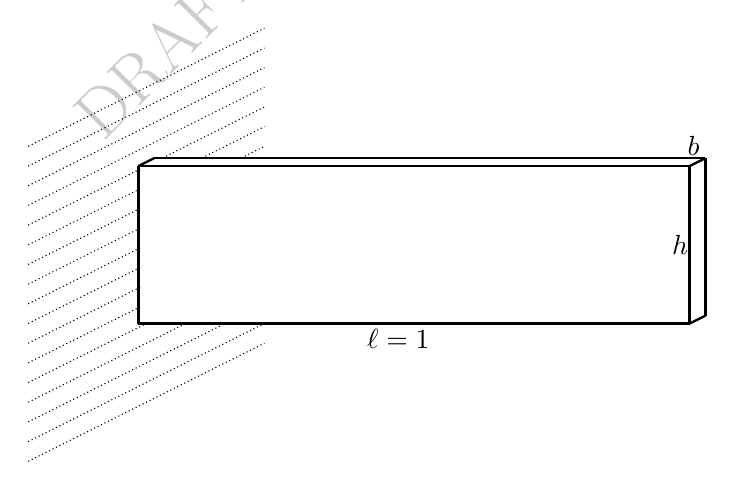
\begin{tikzpicture}
					\draw[line width = 0.3mm] (-0.1,1) -- (6.9,1);
					\draw[line width = 0.3mm] (-0.1,-1) -- (6.9,-1);
					\draw[line width = 0.3mm] (6.9,-1) -- (6.9,1);
					\draw[line width = 0.3mm] (-0.1,-1) -- (-0.1,1);
					
					\draw[line width = 0.3mm] (0.1,1.1) -- (7.1,1.1);
					\draw[line width = 0.3mm] (7.1,-0.9) -- (7.1,1.1);
					
					\draw[line width = 0.3mm] (-0.1,1) -- (0.1,1.1);
					\draw[line width = 0.3mm] (6.9,1) -- (7.1,1.1);
					\draw[line width = 0.3mm] (6.9,-1) -- (7.1,-0.9);
					
					
					
					\draw[scale=0.5, domain=-3:3, smooth, variable=\x,densely dotted] plot ({\x}, {0.5*\x+4});
					\draw[scale=0.5, domain=-3:3, smooth, variable=\x,densely dotted] plot ({\x}, {0.5*\x+3.5});
					\draw[scale=0.5, domain=-3:3, smooth, variable=\x,densely dotted] plot ({\x}, {0.5*\x+3});
					\draw[scale=0.5, domain=-3:3, smooth, variable=\x,densely dotted] plot ({\x}, {0.5*\x+2.5});
					
					\draw[scale=0.5, domain=-3:-0.1, smooth, variable=\x,densely dotted] plot ({\x}, {0.5*\x+2});
					\draw[scale=0.5, domain=-3:-0.1, smooth, variable=\x,densely dotted] plot ({\x}, {0.5*\x+1.5});
					\draw[scale=0.5, domain=-3:-0.1, smooth, variable=\x,densely dotted] plot ({\x}, {0.5*\x+1});
					
					\draw[scale=0.5, domain=0.5:3, smooth, variable=\x,densely dotted] plot ({\x}, {0.5*\x+2});
					\draw[scale=0.5, domain=1.5:3, smooth, variable=\x,densely dotted] plot ({\x}, {0.5*\x+1.5});
					\draw[scale=0.5, domain=2.5:3, smooth, variable=\x,densely dotted] plot ({\x}, {0.5*\x+1});
					
					\draw[scale=0.5, domain=-3:-0.1, smooth, variable=\x,densely dotted] plot ({\x}, {0.5*\x+0.5});
					\draw[scale=0.5, domain=-3:-0.1, smooth, variable=\x,densely dotted] plot ({\x}, {0.5*\x});
					\draw[scale=0.5, domain=-3:-0.1, smooth, variable=\x,densely dotted] plot ({\x}, {0.5*\x-0.5});
					\draw[scale=0.5, domain=-3:-0.1, smooth, variable=\x,densely dotted] plot ({\x}, {0.5*\x-1});
					\draw[scale=0.5, domain=-3:-0.1, smooth, variable=\x,densely dotted] plot ({\x}, {0.5*\x-1.5});
					\draw[scale=0.5, domain=-3:0, smooth, variable=\x,densely dotted] plot ({\x}, {0.5*\x-2});
					\draw[scale=0.5, domain=-3:1, smooth, variable=\x,densely dotted] plot ({\x}, {0.5*\x-2.5});
					\draw[scale=0.5, domain=-3:2, smooth, variable=\x,densely dotted] plot ({\x}, {0.5*\x-3});
					\draw[scale=0.5, domain=-3:3, smooth, variable=\x,densely dotted] plot ({\x}, {0.5*\x-3.5});
					\draw[scale=0.5, domain=-3:3, smooth, variable=\x,densely dotted] plot ({\x}, {0.5*\x-4});
					
					\node at (6.95,1.25) {$b$};
					\node at (6.78,0) {$h$};
					\node at (3.2,-1.2) {$\ell = 1$};
				\end{tikzpicture}
				
			\end{minipage}
		}
    }
\end{figure}


\subsection{Calculating the eigenvalues}
In Section \ref{sec:FEM:3D}, the Finite Element Method for the three-dimensional beam is derived. Similar to the two-dimensional case in \ref{sec:validity-of-a-cantilever-timoshenko-beam}, the Finite Element Method is used to calculate the eigenvalues of the three-dimensional beam. The eigenvalue problem for both models have the same form, but different matrices.

\subsubsection{Problem 2DE and 3D-1E}
Find a real number $\lambda$ and a function $\bar{u} \in S^h$ such that
\begin{eqnarray}
	K\bar{u} & = & M\lambda{\bar{u}},
\end{eqnarray} where $K$ and $M$ are the standard Finite Element Method matrices defined in Section \ref{ssec:2DFEM:DE} for the Problem 2DE and Section \ref{3d_fem_g} for Problem 3DE.

\subsubsection{Accuracy of the eigenvalues of the three-dimensional model}
Figure \ref{fig:conv_3d_eig} show the rate of convergence of the first 20 eigenvalues of Problem 3DE. 

\begin{figure}[H]
    \centering
        \includegraphics[scale=0.7]{files/Chapter6/convergence3d.png}

    \label{fig:conv_3d_eig}
\end{figure}

Similar to the two-dimensional case, the number of elements can be chosen so that at least the first 20 eigenvalues are accurate to 4 significant digits.

For the three-dimensional model, obtaining this level of accuracy can be difficult and computationally expensive. For the two-dimensional beam in Section \ref{sec:validity-of-a-cantilever-timoshenko-beam} and the upcoming two-dimensional plate model in Section \ref{sec:validity-of-a-plate} it is easier to get 5 significant digits of accuracy.

\subsection{Comparing the mode shapes}
To be able to compare the eigenvalues, the mode shapes of the two models are compared to match up the eigenvalues of the two models. This is the same approach as in Section \ref{sec:validity-of-a-cantilever-timoshenko-beam}. 

As seen in Section \ref{sec:validity-of-a-cantilever-timoshenko-beam}, the two-dimensional model as eigenvalues and eigenvectors that are not related to beam type problems. This is also true for the three-dimensional model, and it has even more non-beam type eigenvalues.

The focus of the investigation remains on beam type problems. Below are some examples of the mode shapes for beam type eigenvalues, mode shapes for non-beam type eigenvalues that are shared between the two and three-dimensional models and also mode shapes for non-beam type eigenvalues that are only present in the three-dimensional model.

\subsubsection{Mode shapes relating to beam type eigenvalues.}
Figure \ref{fig:beam-2dv3d} show some examples of beam type mode shapes for the displacement $u$.

\begin{figure}[h!]
	\scalebox{.8}{
		\makebox[\textwidth][c]{
			\centering
			\begin{minipage}[b]{0.8\linewidth}
				\includegraphics[width=1\linewidth]{files/Chapter6/3D12.png}
			\end{minipage}
			\begin{minipage}[b]{0.8\linewidth}
				\includegraphics[width=1\linewidth]{files/Chapter6/2D3.png}
			\end{minipage}
	    }
    }
	\scalebox{.8}{
		\makebox[\textwidth][c]{
			\centering
			\begin{minipage}[b]{0.8\linewidth}
				\includegraphics[width=1\linewidth]{files/Chapter6/3D22.png}
			\end{minipage}
			\begin{minipage}[b]{0.8\linewidth}
				\includegraphics[width=1\linewidth]{files/Chapter6/2D6.png}
			\end{minipage}
	    }
    }
\end{figure}


\subsubsection{Mode shapes relating to non-beam type eigenvalues that are present in the two-dimensional model.}
Figure \ref{fig:nonbeam-2dv3d} show examples of mode shapes relating to non-beam type eigenvalues for the displacement $u$.


\begin{figure}[h!]
	\scalebox{.8}{
		\makebox[\textwidth][c]{
			\centering
			\begin{minipage}[b]{0.8\linewidth}
				\includegraphics[width=1\linewidth]{files/Chapter6/3D33.png}
			\end{minipage}
			\begin{minipage}[b]{0.8\linewidth}
				\includegraphics[width=1\linewidth]{files/Chapter6/2D8.png}
			\end{minipage}
	    }
    }
\end{figure}


\subsubsection{Mode shapes relating to non-beam type eigenvalues that are not present in the two-dimensional model.}
Figure \ref{fig:nonbeam-2dv3d} show examples of mode shapes relating to non-beam type eigenvalues for the displacement $u$ which are not present in the two-dimensional model. These mode shapes only appear in the three-dimensional beam.

\begin{figure}[h!]
	\scalebox{.8}{
		\makebox[\textwidth][c]{
			\centering
			\begin{minipage}[b]{0.8\linewidth}
				\includegraphics[width=1\linewidth]{files/Chapter6/3DNonBeam10.png}
			\end{minipage}
			\begin{minipage}[b]{0.8\linewidth}
				\includegraphics[width=1\linewidth]{files/Chapter6/3DNonBeam11.png}
			\end{minipage}
        }
    }
\end{figure}


\subsection{Comparing the eigenvalues}

For a realistic comparison of the models, the parameters need to be chosen carefully. The parameters are $h$ representing the height of the beam and $b$ representing the width of the beam. The two-dimensional model does not have the width parameter.

For $h$, the values used in Section \ref{sec:validity-of-a-cantilever-timoshenko-beam} will be used. These values covers a range of beam shapes from a short thick beam, to a long slender beam. two cases are selected that represents realistic cases. For a short and thick beam, consider $h = 1/5$ and for a long and slender beam, consider $h = 1/20$.

For the parameter $b$, two different cases will be considered. The first case is for $b \leq h$, and the $b > h$. The distinction of these two cases will become apparent in the results. It is important to note that the parameter $b$ will be expressed as a multiple of $h$.

All of the results will include all the eigenvalues shared between the two-models, including not beam type eigenvalues. The non-beam type eigenvalues will be highlighted in grey. The non-beam type eigenvalues that are not shared between the two models will be excluded from the results, but the numbering of the eigenvalues will be kept as if they were included.

\subsubsection*{Case $b \leq h$:}
Table \ref{tab:2v3_1} below compares the eigenvalues of the models for a beam with a small length to height ratio of $h=1/5$ with decreasing values of $b$. 

\begin{table}[htbp]
	\scalebox{.8}{
	\makebox[\textwidth]{
		\begin{tabular}{|cc|cc|cc|cc||cc|}
			\hline
			\multicolumn{10}{|c|}{Eigenvalues} \\
			\hline
			\hline
			i     & {b = h} & i     & {b = 1/2 h} & i     & {b = 1/4 h} & i     & {b = 1/8 h} & j     & 2D \\
			\hline
			{2} & 0.12307 & {2} & 0.12234 & {2} & 0.12198 & {3} & 0.12178 & 1     & 0.12151 \\
			{3} & 3.5773 & {5} & 3.5630 & {6} & 3.5558 & {8} & 3.5519 & 2     & 3.5460 \\
			\rowcolor{lightgray}{5} & 7.7799 & {6} & 7.7596 & {8} & 7.7471 & {11} & 7.7401 & 3     & 7.7311 \\
			{8} & 20.334 & {9} & 20.283 & {11} & 20.26 & {14} & 20.247 & 4     & 20.225 \\
			{10} & 56.247 & {12} & 56.173 & {15} & 56.156 & {22} & 56.142 & 5     & 56.109 \\
			\rowcolor{lightgray}{11} & 69.197 & {14} & 69.319 & {17} & 69.281 & {24} & 69.238 & 6     & 69.164 \\
			{14} & 114.03 & {16} & 114.01 & {20} & 114.05 & {29} & 114.06 & 7     & 114.03 \\
			\rowcolor{lightgray}{17} & 187.01 & {19} & 189.14 & {25} & 189.37 & {36} & 189.34 & 8     & 189.17 \\
			{18} & 192.21 & {20} & 192.41 & {26} & 192.58 & {37} & 192.63 & 9     & 192.61 \\
			{21} & 284.76 & {23} & 285.43 & {31} & 285.74 & {42} & 285.84 & 10    & 285.85 \\
			{23} & 327.57 & {26} & 328.24 & {35} & 328.37 & {46} & 328.40 & 11    & 328.40 \\
			\rowcolor{lightgray}{25} & 347.77 & {28} & 356.44 & {36} & 357.30 & {50} & 357.33 & 12    & 357.08 \\
			{27} & 393.69 & {30} & 396.84 & {38} & 397.28 & {53} & 397.37 & 13    & 397.33 \\
			{30} & 434.46 & {34} & 441.05 & {41} & 441.81 & {57} & 441.99 & 14    & 442.00 \\
			\rowcolor{lightgray}{31} & 523.65 & {36} & 534.04 & {43} & 534.17 & {63} & 534.03 & 15    & 533.71 \\
			{34} & 550.51 & {37} & 537.82 & {44} & 538.86 & {64} & 539.06 & 16    & 538.97 \\
			\rowcolor{lightgray}{37} & 590.86 & {41} & 587.43 & {48} & 594.17 & {65} & 595.58 & 17    & 596.06 \\
			{39} & 590.86 & {42} & 600.52 & {49} & 602.25 & {67} & 602.69 & 18    & 602.77 \\
			\rowcolor{lightgray}{42} & 646.21 & {44} & 657.22 & {50} & 658.04 & {71} & 658.06 & 19    & 657.87 \\
			{44} & 711.07 & {46} & 714.62 & {53} & 717.10 & {73} & 717.51 & 20    & 717.37 \\
			\hline
			\hline
			\multicolumn{2}{|c|}{Max RE: \  2.6069\%} &\multicolumn{2}{c|}{Max RE: \ 1.4469\%}  & \multicolumn{2}{c|}{Max RE: \  0.38192\%}  & \multicolumn{2}{c||}{Max RE: \ 0.22301\%}& \multicolumn{2}{c|}{-} \\
			\hline
		\end{tabular}
	    }
    }
\end{table}%

\label{sym:RE}

% Table generated by Excel2LaTeX from sheet 'Sheet2'
\begin{table}[htbp]
	\centering
	\begin{tabular}{|c|cccc|}
		\hline
		\multicolumn{5}{|c|}{Maximum Relative Error} \\
		\hline
		\hline
		& {b = h} & {b = 1/2h} & {b = 1/4h} & {b = 1/8h} \\
		\hline
		Beam Type & 2.1420 \% & 0.6804 \% & 0.38192 \% & 0.22301 \% \\
		Non-Beam Type & 2.6069 \% & 1.4469 \% & 0.31546 \% & 0.11680 \% \\
		\hline
	\end{tabular}%
	\label{tab:2Dv3D_1_breakup}%
\end{table}%

Table \ref{tab:2v3_1} below compares the eigenvalues of the models for a beam with a larger length to height ratio of $h=1/20$ with decreasing values of $b$. 

\begin{table}[ht]
	\scalebox{.8}{
	\makebox[\textwidth]{
	\begin{tabular}{|cc|cc|cc|cc||cc|}
		\hline
		\multicolumn{10}{|c|}{Eigenvalues} \\
		\hline
		\hline
		i     & {b = h} & i     & {b = 1/2 h} & i     & {b = 1/4 h} & i     & {b = 1/8 h} & j     & 2D \\
		\hline
		{2} & 0.008043 & {2} & 0.008029 & {2} & 0.008023 & {3} & 0.00802 & {1} & {0.008013} \\
		{3} & 0.3087 & {4} & 0.30816 & {5} & 0.30794 & {7} & 0.30785 & {2} & {0.30757} \\
		{5} & 2.3357 & {8} & 2.3316 & {9} & 2.3300  & {12} & 2.3293 & {3} & {2.3273} \\
		\rowcolor{lightgray}{8} & 7.7217 & {10} & 7.7156 & {13} & 7.7124 & {16} & 7.7111 & {4} & {7.7077} \\
		{10} & 8.5387 & {11} & 8.5238 & {14} & 8.5182 & {18} & 8.516 & {5} & {8.5086} \\
		{11} & 21.986 & {14} & 21.948 & {18} & 21.934 & {24} & 21.929 & {6} & {21.911} \\
		{14} & 45.863 & {18} & 45.781 & {21} & 45.756 & {30} & 45.746 & {7} & {45.712} \\
		\rowcolor{lightgray}{17} & 69.444 & {19} & 69.408 & {25} & 69.385 & {33} & 69.374 & {8} & {69.344} \\
		{18} & 83.149 & {22} & 82.999 & {27} & 82.960 & {36} & 82.944 & {9} & {82.887} \\
		{21} & 136.44 & {25} & 136.19 & {31} & 136.14 & {42} & 136.12 & {10} & {136.03} \\
		\rowcolor{lightgray}{23} & 192.62 & {27} & 192.62 & {35} & 192.58 & {47} & 192.56 & {11} & {192.48} \\
		{25} & 207.87 & {29} & 207.5 & {36} & 207.43 & {48} & 207.41 & {12} & {207.29} \\
		{27} & 299.14 & {33} & 298.63 & {41} & 298.56 & {55} & 298.53 & {13} & {298.38} \\
		\rowcolor{lightgray}{30} & 376.68 & {35} & 377.01 & {44} & 377.01 & {58} & 376.98 & {14} & {376.83} \\
		{31} & 411.58 & {37} & 410.89 & {46} & 410.83 & {61} & 410.81 & {15} & {410.63} \\
		{34} & 546.15 & {40} & 545.27 & {50} & 545.24 & {66} & 545.23 & {16} & {545.03} \\
		\rowcolor{lightgray}{37} & 620.77 & {42} & 622.02 & {53} & 622.19 & {69} & 622.18 & {17} & {621.95} \\
		{39} & 703.55 & {44} & 702.49 & {54} & 702.29 & {71} & 702.53 & {18} & {702.31} \\
		{42} & 884.27 & {47} & 883.02 & {59} & 883.14 & {82} & 883.19 & {19} & {882.96} \\
		\rowcolor{lightgray}{44} & 923.68 & {49} & 926.88 & {60} & 927.43 & {86} & 927.50 & {20} & {927.18} \\
		\hline
		\hline
		\multicolumn{2}{|c|}{Max RE: \  0.37701\%} &\multicolumn{2}{c|}{Max RE: \ 0.19893\%}  & \multicolumn{2}{c|}{Max RE: \  0.12393\%}  & \multicolumn{2}{c||}{Max RE: \ 0.092843\%}& \multicolumn{2}{c|}{-} \\
		\hline
	\end{tabular}%
	\label{tab:2v3_2}%
    }
}
\end{table}%


\begin{table}[htbp]
	\centering

	\begin{tabular}{|c|cccc|}
		\hline
		\multicolumn{5}{|c|}{Maximum Relative Error} \\
		\hline
		\hline
		& {b = h} & {b = 1/2h} & {b = 1/4h} & {b = 1/8h} \\
		\hline
		Beam Type & 0.37701 \% & 0.19893 \% & 0.12393 \% & 0.092843 \% \\
		Non-Beam Type & 0.37682 \% & 0.10218 \% & 0.061213 \% & 0.043601 \% \\
		\hline
	\end{tabular}%
	\label{tab:2v3_2_split}%
\end{table}%


Tables \ref{tab:2v3_1} and \ref{tab:2v3_2} show that the first 20 eigenvalues two-dimensional model compares very well to the matching eigenvalues three-dimensional beam for $b<=h$. As the width $b$ decreases, the two-dimensional model becomes a better approximation of the three-dimensional model. Also shown is that the slender beam with $h = 1/20$ compares better than the thick beam where $h = 1/5$, event though the case of $h=1/5$ is still a very good comparison. 

The tables also shows that the three-dimensional model has more non-beam type eigenvalues as the width $b$ decreases, as well as when the width $h$ decreases.This is different from the two-dimensional model as seen in \ref{sec:validity-of-a-cantilever-timoshenko-beam}.

Tables \ref{tab:2Dv3D_1_breakup} and \ref{tab:2v3_2_split} breaks up the maximum relative error for the beam type and non-beam type eigenvalues. These tables confirm that the the beam type eigenvalues compare very well.


\subsubsection*{Case $b > h$:}
First, the case is considered where $h = 1/5$.


\begin{table}[htbp]
	\scalebox{.8}{
	\makebox[\textwidth]{
		\begin{tabular}{|cc|cc|cc||cc|}
			\hline
			\multicolumn{8}{|c|}{Eigenvalues} \\
			\hline
			\hline
			i     & {b = 2h} & i     & {b = 4h} & i     & {b = 8h} & j     & 2D \\
			\hline
			{1} & 0.12474 					& {1} & 0.12766 & {1} & 0.13036 & 1     & 0.12151 \\
			{4} & 3.6088 					& {4} & 3.6297 & {5} & 3.7766 & 2     & 3.5460 \\
			\rowcolor{lightgray}{6} & 7.8091 & {5} & 7.8389 & {9} & 8.9239 & 3     & 7.7311 \\
			{8} & 20.466 					& {9} & 20.959 & {15} & 21.031 & 4     & 20.255 \\
			{11} & 56.309					& {18} & 58.149 & {30} & 60.862 & 5     & 56.109 \\
			\hline
			\hline
			\multicolumn{2}{|c|}{Max RE: \  2.6603\%} &\multicolumn{2}{c|}{Max RE: \ 5.0571\%}  & \multicolumn{2}{c|}{Max RE: \  15.428\%} & \multicolumn{2}{c|}{-} \\
			\hline
		\end{tabular}%
		\label{tab:b>h}%
	    }
    }
\end{table}



\begin{table}[htbp]
	\centering

	\begin{tabular}{|c|ccc|}
		\hline
		\multicolumn{4}{|c|}{Maximum Relative Error} \\
		\hline
		\hline
		& {b = 2h} & {b = 4h} & {b = 8h} \\
		\hline
		Beam Type & 2.6603 \% & 5.0571 \% & 8.4712 \% \\
		Non-Beam Type & 1.0096 \% & 1.3948 \% & 15.428 \% \\
		\hline
	\end{tabular}%
	\label{tab:b>h-split}%
\end{table}%


In Table \ref{tab:b>h}, the height of the beam is set to $h=1/20$, which was the best case when $b<h$.


\begin{table}[htbp]
	\scalebox{.8}{
	\makebox[\textwidth]{
		\begin{tabular}{|cc|cc|cc||cc|}
			\hline
			\multicolumn{8}{|c|}{Eigenvalues} \\
			\hline
			\hline
			i     & {b = 2h} & i     & {b = 4h} & i     & {b = 8h} & j     & 2D \\
			\hline
			{2} & 0.008076 & {1} & 0.008162 & {1} & 0.008324 & 1     & 0.008013 \\
			{3} & 0.30995 & {3} & 0.31298 & {3} & 0.31738 & 2     & 0.30757 \\
			{5} & 2.3462 & {5} & 2.3737 & {6} & 2.4116 & 3     & 2.3273 \\
			\rowcolor{lightgray}{8} & 7.7312 & {8} & 7.7471 & {9} & 7.7711 & 4     & 7.7077 \\
			{10} & 8.5841 & {9} & 8.7082 & {10} & 8.7929 & 5     & 8.5086 \\
			{11} & 22.124 & {12} & 22.491 & {14} & 23.222 & 6     & 21.911 \\
			{14} & 46.195 & {14} & 47.003 & {18} & 47.921 & 7     & 45.712 \\
			\rowcolor{lightgray}{17} & 69.454 & {17} & 69.281 & {22} & 72.307 & 8     & 69.344 \\
			{18} & 83.822 & {18} & 85.218 & {24} & 80.607 & 9     & 82.887 \\
			{21} & 137.43 & {21} & 138.58 & {32} & 140.97 & 10    & 136.03 \\
			\hline
			\hline
			\multicolumn{2}{|c|}{Max RE: \  1.1289\%} &\multicolumn{2}{c|}{Max RE: \ 2.8261\%}  & \multicolumn{2}{c|}{Max RE: \  5.9821\%} & \multicolumn{2}{c|}{-} \\
			\hline
		\end{tabular}%
	    }
    }
\end{table}



\begin{table}[htbp]
	\centering
	
	\begin{tabular}{|c|ccc|}
		\hline
		\multicolumn{4}{|c|}{Maximum Relative Error} \\
		\hline
		\hline
		& {b = 2h} & {b = 4h} & {b = 8h} \\
		\hline
		Beam Type & 1.1289 \% & 2.8261 \% & 5.9821 \% \\
		Non-Beam Type & 0.30521 \% & 0.51096 \% & 4.2734 \% \\
		\hline
	\end{tabular}%
	\label{tab:b>h-split_20}%
\end{table}%


Tables \ref{tab:b>h} and \ref{tab:b>h_20} show that the two-dimensional model compares less well to the three-dimensional model when $b$ is too much larger than $h$. Tables \ref{tab:b>h-split} and \ref{tab:b>h-split_20} show that this is also true for the beam type eigenvalues.

For the case of $h=1/5$, it was also more difficult to obtain reliable eigenvalues using a numerical method.

These results gives a detailed overview of the validity of the cantilever two-dimensional beam compared to the cantilever three-dimensional beam. The results show that the two-dimensional beam model compares very well to the three-dimensional beam model for a large range of beam shapes. The results shown were chosen to represent realistic cases, and the results are similar for other cases.

The overall conclusion is that the shape of the beam is very important. If the width $b$ is equal to or less than the height $h$, the two-dimensional beam model compares very well to the three-dimensional beam model. More so when the beam is slender, and less so when the beam is short and thick.

When the width $b$ is larger than the height $h$, the two-dimensional beam the comparison degrades very quickly. This is true for both slender and short and thick beams, although with short and thick beams, it is more difficult to obtain reliable eigenvalues using a numerical method.

For practical applications, if $b > h$ the use of a beam model must be brought into question. Other models such as a plate model will be better suited as it is a more realistic model. In the next section, the validity of the Reissner-Mindlin plate mode is investigated using the same method of this section.


\section{Conclusion}
his chapter is an extension of the work of Section 4.5. In Section 4.5, the validity of the Timoshenko beam theory is investigated by comparing a Timoshenko beam model to a two-dimensional beam model. 

In real-world applications, a beam is a three-dimensional model. Therefore it should be more realistic to use a three-dimensional model to investigate the validity of the Timoshenko beam theory. This is mentioned by the authors of \cite{LVV09}. Their suggestion is to use the two-dimensional model as an intermediate step, to avoid complexities. Therefore the validity of the two-dimensional model is investigated, using a three-dimensional beam model as a reference. Again the results so that the comparison relies on the shape of the beams. The two-dimensional model compares well to the three-dimensional beam if the beam is not wide. 

If the width of the beam is very large, the use of a beam model can be questioned. A plate model might be more suited. Therefore the last section of this chapter investigates the validity of the Reissner-Mindlin plate model. The Reissner-Mindlin plate model is compared to a three-dimensional plate model. The results show that the Reissner-Mindlin plate model compares well to the three-dimensional plate model.

The same method is used in this chapter as in Section 4.5. The mode shapes are sketched and matched. The corresponding eigenvalues can then be matched up and compared. The eigenvalues relating to the Reissner-Mindlin plate model are referred to as plate-type eigenvalues.

\section{Contributions}

There are four models used in this dissertation. For each of the models, the dimensionless variational form is derived. Also presented are the model problems that are used in this dissertation.

The first result investigates the existence and uniqueness of solutions for general vibration problems. The article that is discussed proves this result for a general vibration problem, using four assumptions. To explain the theory, an example is presented using one of the model problems of the dissertation. The cantilever Timoshenko beam model is chosen for the simple boundary conditions, as well as it's recurring importance in this dissertation. The weak variational form of the model is derived as well as the function spaces defined. This is presented in the same format as the general vibration problem. In fact all the models in this dissertation are special cases of this general vibration problem. The theory is then applied to this example problem, as a demonstration. To apply the theory, the four assumptions are proven to be true.

The next result looks at modal analysis. Before the general case is discussed, again the cantilever Timoshenko beam is used to illustrated the concept of modal analysis.A trial solution to the boundary value problem is suggested. This trial solution is substituted into the partial differential equation and two problems are obtained. The first problem is the eigenvalue problem and the second is an ordinary differential equation. The eigenvalue problem can be solved with theory discussed later in the dissertation and the ordinary differential equation can then be solved. Substation of these two results into the boundary value problem confirms that the trial solution is correct. The same idea is then discussed for the general case.

We then look at the convergence of the Galerkin Approximation for our general vibration problem. The results of the article discussed are updated with improved notation using a different article. The general case of the Galerkin approximation use a lot of symbols that are not immediately obvious, so again the cantilever Timoshenko beam model problem is used and the Galerkin Approximation is derived in an attempt to explain some of the conventions. The results of the article are then discussed and presented. The results are presented in a concise and practical format to reduce the need to define any unnecessary symbols or notation. The results are also presented in four theorems, summarizing the results of the article that are important but that are not necessarily presented as a theorem in the article.

The next result is on the convergence of the eigenvalues and eigenfunctions of a general vibration problem when using the Finite Element Method. The results are from a textbook. The results are presented with updated notation, coinciding with the notation used in the dissertation. The results are also expanded and extra results are added in an attempt to better explain the theory.

We then look at an important result for the Timoshenko beam theory. This provides a method to calculate the exact eigenvalues and eigenfunctions for the Timoshenko beam theory. Two examples are then used, a cantilever beam and a free-free beam, as an example of the application of the theory. The eigenvalues are calculated and the corresponding mode shapes are plotted. To obtain these results, the equation of motion is plotted, the isolation intervals are determined and the eigenvalues are then calculated using interval division to a desired level of accuracy. The mode shapes can then also be plotted with back substitution. These examples are important preparation for the main comparisons of this dissertation. We also discuss a result comparing the Timoshenko beam theory to results from an empirical study. We add to this article by giving the model problems.

For the rest of the models in this dissertation, the two- and three-dimensional elastic bodies, and the Reissner-Mindlin plate model, a different approach is required to solve the eigenvalue problems. For these models we use the Finite Element Method. For each of the models, their reference configurations are given. All of the models are assumed to have a square cross-section and in a cantilever configuration. This reference configuration is then discretised into a grid of rectangular shaped elements. A set of admissable piecewise Hermite cubic functions are then used and each model is rewritten into a Galerkin Approximation. We the define the standard Finite Element Method Matrices for each case. These are referred to as the mass and stiffness matrices in engineering. Finally our boundary value problems are written into a system of ordinary differential equations in a matrix representation. At this point is it easy to derive the eigenvalue problem for each of the problems in this matrix form. This is in preparation for the main comparisons made in this dissertation. 

For our main comparisons, we first look at an article comparing a cantilever Timoshenko beam model to a cantilever two-dimensional model. We discuss the article and replicate the results. The eigenvalues and eigenfunctions of the Timoshenko beam model is obtained using the exact method already described. The eigenvalues and the eigenfunctions for the two-dimensional model are approximated using the Finite Element Method matrix representation of the eigenvalue problem. A MATLAB program is written to approximate the eigenvalues and plot the mode shapes. The accuracy of this approximation is also investigated by looking at the rate of convergence for different grid sizes. Following the article, the eigenvalues are matched up by first comparing the mode shapes of the two models. The eigenvalues can then be matched up and also any eigenvalues not relating to beam-type problems can be filtered out. Based on the results in modal analysis, only a few eigenvalues need to be considered. The relative error between the eigenvalues are then calculated for different shapes of beams. The results improve on the article by showing more significant digits and also including some more results. 

We then extend the results of the article to investigate the validity of a cantilever two-dimensional beam model as well as a cantilever Reissner-Mindlin plate model. The same method of the article is followed. To investigate the validity of a cantilever two-dimensional model, a cantilever three-dimensional model is considered. Since both of the models are not beam models, careful consideration needs to be taken to identify the eigenvalues. The same approach is used by comparing the mode shapes. For interest, the non-beam type eigenvalues shared between the two models are also included and the rest that the three-dimensional model does not share with the two-dimensional model are omitted. A clear distinction is made to show the beam type eigenvalues and the beam type results. The shape of the models are also carefully chosen to represent a variety of realistic cases that are interesting. The results show that the shape of the models play an important role in how well the models compare. An interesting result shows that this comparison is not good when the beam gets too wide. We therefore suggest a different model, like a plate model. This lead to the introduction of the Reissner-Mindlin plate model into this dissertation. The validity of a cantilever Reissner-Mindlin plate model is investigated using the same method. The cantilever three-dimensional plate model is again used as the reference model with the restriction that the body is wide.


\section*{References}
\bibliographystyle{plainnat}
\bibliography{references.bib}

\end{document}